% Options for packages loaded elsewhere
\PassOptionsToPackage{unicode}{hyperref}
\PassOptionsToPackage{hyphens}{url}
%
\documentclass[
]{article}
\usepackage{amsmath,amssymb}
\usepackage{iftex}
\ifPDFTeX
  \usepackage[T1]{fontenc}
  \usepackage[utf8]{inputenc}
  \usepackage{textcomp} % provide euro and other symbols
\else % if luatex or xetex
  \usepackage{unicode-math} % this also loads fontspec
  \defaultfontfeatures{Scale=MatchLowercase}
  \defaultfontfeatures[\rmfamily]{Ligatures=TeX,Scale=1}
\fi
\usepackage{lmodern}
\ifPDFTeX\else
  % xetex/luatex font selection
\fi
% Use upquote if available, for straight quotes in verbatim environments
\IfFileExists{upquote.sty}{\usepackage{upquote}}{}
\IfFileExists{microtype.sty}{% use microtype if available
  \usepackage[]{microtype}
  \UseMicrotypeSet[protrusion]{basicmath} % disable protrusion for tt fonts
}{}
\makeatletter
\@ifundefined{KOMAClassName}{% if non-KOMA class
  \IfFileExists{parskip.sty}{%
    \usepackage{parskip}
  }{% else
    \setlength{\parindent}{0pt}
    \setlength{\parskip}{6pt plus 2pt minus 1pt}}
}{% if KOMA class
  \KOMAoptions{parskip=half}}
\makeatother
\usepackage{xcolor}
\usepackage{longtable,booktabs,array}
\usepackage{multirow}
\usepackage{calc} % for calculating minipage widths
% Correct order of tables after \paragraph or \subparagraph
\usepackage{etoolbox}
\makeatletter
\patchcmd\longtable{\par}{\if@noskipsec\mbox{}\fi\par}{}{}
\makeatother
% Allow footnotes in longtable head/foot
\IfFileExists{footnotehyper.sty}{\usepackage{footnotehyper}}{\usepackage{footnote}}
\makesavenoteenv{longtable}
\usepackage{graphicx}
\makeatletter
\newsavebox\pandoc@box
\newcommand*\pandocbounded[1]{% scales image to fit in text height/width
  \sbox\pandoc@box{#1}%
  \Gscale@div\@tempa{\textheight}{\dimexpr\ht\pandoc@box+\dp\pandoc@box\relax}%
  \Gscale@div\@tempb{\linewidth}{\wd\pandoc@box}%
  \ifdim\@tempb\p@<\@tempa\p@\let\@tempa\@tempb\fi% select the smaller of both
  \ifdim\@tempa\p@<\p@\scalebox{\@tempa}{\usebox\pandoc@box}%
  \else\usebox{\pandoc@box}%
  \fi%
}
% Set default figure placement to htbp
\def\fps@figure{htbp}
\makeatother
\ifLuaTeX
  \usepackage{luacolor}
  \usepackage[soul]{lua-ul}
\else
  \usepackage{soul}
\fi
\setlength{\emergencystretch}{3em} % prevent overfull lines
\providecommand{\tightlist}{%
  \setlength{\itemsep}{0pt}\setlength{\parskip}{0pt}}
\setcounter{secnumdepth}{2} % number sections and subsections (as in the Word manual)
\setcounter{tocdepth}{2}
\usepackage[margin=1in]{geometry}
\usepackage{fancyhdr}
\pagestyle{fancy}
\fancyhf{}
\fancyhead[L]{BridgeTrafficLoadSim (v1.3.8)}
\fancyhead[R]{User Manual}
\fancyfoot[C]{\thepage}
\fancyfoot[R]{\footnotesize © Colin Caprani 2012--26}
\renewcommand{\headrulewidth}{0.4pt}
\usepackage{bookmark}
\IfFileExists{xurl.sty}{\usepackage{xurl}}{} % add URL line breaks if available
\urlstyle{same}
\hypersetup{
  hidelinks,
  pdfcreator={LaTeX via pandoc}}

\author{}
\date{}

\begin{document}

\begin{titlepage}
\centering
{\LARGE\bfseries BridgeTrafficLoadSim:}\\[0.5em]
{\Large\emph{Long Run Simulation Model}}\\[0.3em]
{\Large\emph{for Bridge Loading}}\\[1.5em]
{\large Version 1.3.8}\\[2em]
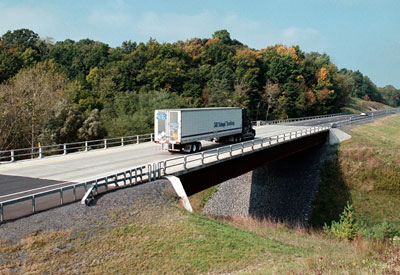
\includegraphics[width=4.1625in,height=2.86042in]{media/image1.jpeg}\\[2em]
{\Large\emph{User Manual}}\\[2em]
{\large Dr Colin Caprani}\\[0.3em]
{\large Monash University}
\vfill
\end{titlepage}

\textbf{Acknowledgements}

This program is based on three separate programs developed as part of
the author's PhD research from 2001. In turn, these were based on work
by Dr Samuel Grave, former PhD student at Trinity College Dublin. The
current program which encompasses the functions of two of the previous
programs has evolved since 2007 and has been much influenced by the work
of Dr Bernard Enright, DIT.

For further information, please contact
\href{mailto:colin.caprani@monash}{\nolinkurl{colin.caprani@monash}}.

Dr Colin Caprani,

July 2012

\newpage

\tableofcontents

\newpage

\section{Introduction}\label{introduction}

\subsection{The BridgeTrafficLoadSim
Program}\label{the-bridgetrafficloadsim-program}

BridgeTrafficLoadSim will be referred to as BTLS hereafter.

BTLS generates artificial traffic and passes it across bridges
determining various load effects. The traffic is generated according to
a relatively simple model. There are several built-in influence lines
for various load effects, but the user can input their own influence
line also. The program outputs various quantities of interest, which are
controllable by the user.

These programs have been in use in DIT and University College Dublin
over a 10-year period. There have been multiple users, and so exhibit a
fair degree of maturity. That is, the user should not get unexpected
results when used correctly. Whilst the routines have been thoroughly
tested many times, with ongoing changes, it is good practice to satisfy
oneself as to the accuracy of the programs. Various forms of output
should assist with this process.

\subsection{The User Manual}\label{the-user-manual}

\subsubsection*{Purpose}\label{purpose}
\addcontentsline{toc}{subsubsection}{Purpose}

This User Manual has been written to explain the use of the BTLS
program, and to explain its capabilities and limitations.

\textbf{Notices}

Points of significant importance are denoted as:

\textbf{\ul{Important!}}

Typically, failure to adhere to these points will result in unexpected
behaviour or a program crash.

\subsubsection*{\texorpdfstring{\hfill\break
Glossary}{ Glossary}}\label{glossary}
\addcontentsline{toc}{subsubsection}{\hfill\break
Glossary}

Load Effect The result of a calculation using any influence line. Total
load on the bridge is sometimes referred to as a load effect therefore.

\subsection{Program Release History}\label{program-release-history}

\begin{longtable}[]{@{}
  >{\centering\arraybackslash}p{(\linewidth - 4\tabcolsep) * \real{0.1298}}
  >{\centering\arraybackslash}p{(\linewidth - 4\tabcolsep) * \real{0.1420}}
  >{\raggedright\arraybackslash}p{(\linewidth - 4\tabcolsep) * \real{0.7282}}@{}}
\toprule\noalign{}
\endhead
\bottomrule\noalign{}
\endlastfoot
\textbf{Version} & \textbf{Date} & \textbf{Description} \\
1.0.0 & 5/7/12 & \begin{minipage}[t]{\linewidth}\raggedright
\begin{itemize}
\item
  Initial release to international users
\end{itemize}
\end{minipage} \\
1.0.1 & 21/7/12 & \begin{minipage}[t]{\linewidth}\raggedright
\begin{itemize}
\item
  Added version number on screen output
\item
  Fixed problem with AllEvents output -- it now outputs the last
  unfilled buffer properly.
\end{itemize}
\end{minipage} \\
1.0.2 & 24/7/12 & \begin{minipage}[t]{\linewidth}\raggedright
\begin{itemize}
\item
  Added a FatigueEvents output file type with max and min values of
  loading events in it. Only output if AllEvents is output - temporarily
\end{itemize}
\end{minipage} \\
1.0.3 & 27/7/12 & \begin{minipage}[t]{\linewidth}\raggedright
\begin{itemize}
\item
  Bug fix: truck departures not always correctly calculated - fixed
  using 1e300 for timeOff variables.
\item
  Bug fix: reading single lane vehicle files caused crash - fixed.
\item
  Minor console output changes for more user information
\end{itemize}
\end{minipage} \\
1.0.4 & 13/8/12 & \begin{minipage}[t]{\linewidth}\raggedright
\begin{itemize}
\item
  Console output for missing files.
\item
  Bug fix: reading multiple lane vehicle files crashed following v1.0.3
  fix for single lanes!
\end{itemize}
\end{minipage} \\
1.0.5 & 27/8/12 & \begin{minipage}[t]{\linewidth}\raggedright
\begin{itemize}
\item
  Separate discrete influence lines now possible for each lane (IL
  option 2 in bridge definition file).
\end{itemize}
\end{minipage} \\
1.1.0 & 27/10/12 & \begin{minipage}[t]{\linewidth}\raggedright
\begin{itemize}
\item
  Peaks over Threshold output
\item
  Basic statistics output
\item
  Created inheritance structure for output types
\item
  Flow Data statistics output
\item
  Restructured the BTLSin file
\item
  Fixed some bugs, especially one on flow generation
\item
  Renamed output files for consistency
\end{itemize}
\end{minipage} \\
1.2.0 & 28/11/12 & \begin{minipage}[t]{\linewidth}\raggedright
\begin{itemize}
\item
  Added Influence Surface (IS) calculations
\item
  Amended BTLSin file structure accordingly
\item
  Added new file structure -- DITIS for ISs, including wheel track width
  for each axle
\item
  Added POT counter file output and input specs in BTLSin
\item
  Program can now run without IL or IS files being present in folder,
  once not required.
\item
  Added option for vehicle output file format
\item
  Traffic folder location now can be specified in BTLSin
\item
  Updated generation of tri-modal-normal distributions to include
  deterministic and single-generation value for axle track widths
\item
  Added transverse position in lane variability through BTLSin
\item
  Added transverse axle track width generation file (ATW.csv) input and
  default value options
\end{itemize}
\end{minipage} \\
1.2.1 & 20/12/12 & \begin{minipage}[t]{\linewidth}\raggedright
\begin{itemize}
\item
  Bug fix: influence surface calculations did not take transverse
  position into account -- now fixed.
\item
  Bug fix: crash caused by traffic files with no vehicles in a lane is
  fixed.
\end{itemize}
\end{minipage} \\
1.2.2 & 27/3/2014 & \begin{minipage}[t]{\linewidth}\raggedright
\begin{itemize}
\item
  Bug fix: VehicleBuffer.h(31) now max axles 20
\item
  Improved feedback on incorrect load effect definitions
\end{itemize}
\end{minipage} \\
1.2.3 & 14/6/2019 & \begin{minipage}[t]{\linewidth}\raggedright
\begin{itemize}
\item
  TH file time precision is now 3 places
\item
  Bridge/IS files now can include comment lines
  `\textbackslash\textbackslash'
\end{itemize}
\end{minipage} \\
1.2.4 & 12/8/2019 & \begin{minipage}[t]{\linewidth}\raggedright
\begin{itemize}
\item
  Added number of events of each truck count to statistics output
\end{itemize}
\end{minipage} \\
1.2.5 & 21/08/19 & \begin{minipage}[t]{\linewidth}\raggedright
\begin{itemize}
\item
  Added MON file format
\item
  Cleaned up all warnings
\item
  Corrected minor bugs in flow/sim time calculations
\end{itemize}
\end{minipage} \\
1.2.6 & 25/08/19 & \begin{minipage}[t]{\linewidth}\raggedright
\begin{itemize}
\item
  Generic classification of vehicles
\item
  Improved warnings
\item
  Clarified local and global lane numberings
\item
  Block numbering fixed to relative sim time
\item
  Correct MON file bug
\end{itemize}
\end{minipage} \\
1.3.0 & 28/08/19 & \begin{minipage}[t]{\linewidth}\raggedright
\begin{itemize}
\item
  Generic flow and vehicle generation routines
\item
  Flow and vehicle models can now be mixed
\item
  Added new garage vehicle generator
\end{itemize}
\end{minipage} \\
1.3.1 & 30/08/19 & \begin{minipage}[t]{\linewidth}\raggedright
\begin{itemize}
\item
  Minor bug fixes (kernels \& RNG seed)
\item
  Started OpenMP, but crashes in x64 release
\item
  Bug fix: RNG seed, and kernels
\item
  Converted to shared\_ptr
\item
  Still has memory leaks in CConfigData
\end{itemize}
\end{minipage} \\
1.3.2 & 2/09/19 & \begin{minipage}[t]{\linewidth}\raggedright
\begin{itemize}
\item
  Fixed CVehicleBuffer bug, storing every vehicle forever.
\item
  Moved input files to Working directory
\item
  clarified memory leak reports
\item
  improved smart pointer useage
\end{itemize}
\end{minipage} \\
1.3.3 & 2/09/19 & \begin{minipage}[t]{\linewidth}\raggedright
\begin{itemize}
\item
  Corrected overlap bug, and improved reporting of potential overlaps
\end{itemize}
\end{minipage} \\
1.3.4 & 3/09/19 & \begin{minipage}[t]{\linewidth}\raggedright
\begin{itemize}
\item
  Fixed bug in MinGap calculations
\item
  Necessary to re-order sequence of start up
\end{itemize}
\end{minipage} \\
1.3.5 & 17/09/19 & \begin{minipage}[t]{\linewidth}\raggedright
\begin{itemize}
\item
  RNG updated to C++11 STL
\item
  Updated Project Configurations: changed exe to x64 default, and now
  x86 is named x86
\item
  More warnings quashed
\item
  Minor performance tweaks
\end{itemize}
\end{minipage} \\
1.3.6 & 20/09/23 & \begin{minipage}[t]{\linewidth}\raggedright
\begin{itemize}
\item
  Use C++17 for the path lib
\item
  Support rainflow process
\item
  Many minor bug fixes for cross-platform compiling
\item
  Add two built-in load effects
\item
  Fix some typos
\end{itemize}
\end{minipage} \\
1.3.7 & 4/7/26 & \begin{minipage}[t]{\linewidth}\raggedright
\begin{itemize}
\item
  Added the SiWIM CSV traffic input file format (format code 5, read
  only)
\item
  Rainflow counting rewritten to the ASTM E1049-85 four-point method;
  cycle counts are no longer dependent on output buffer size
\item
  Statistics output fixes: interval column alignment, added Min/Max
  columns, and trailing quiet blocks/intervals are now written up to
  the simulated end time
\item
  Bug fix: lanes with a zero-flow hour are no longer permanently
  silenced for the rest of the simulation
\item
  Approximately 1.8$\times$ faster single-core execution through I/O
  and copy improvements (bit-exact outputs)
\item
  If \texttt{BTLSin.txt} cannot be opened the program now reports an
  error and exits with a non-zero code, instead of proceeding with
  default values
\item
  Removed the Windows-only ``PAUSE'' console prompts; the program exits
  cleanly on all platforms and returns a proper exit code
\item
  The console banner now reports the actual build version
\end{itemize}
\end{minipage} \\
1.3.8 & 7/9/26 & \begin{minipage}[t]{\linewidth}\raggedright
\begin{itemize}
\item
  Bug fix (changes results): the Grave vehicle model drew the GVW of
  trucks in direction-1 lanes from the direction-2 distribution, because
  the lane direction was never passed to the generator
\item
  Bug fix (changes results): the congested headway model used the gap
  coefficient of variation (Line 12) as an absolute standard deviation
  in seconds; it is again relative to the mean congested gap
\item
  Bug fix: the nominal (constant) vehicle model applied the axle-spacing
  and axle-weight coefficients of variation to each other's quantity
\item
  A run with load effects enabled but an empty bridge file no longer sets
  the no-overlap length to 0 m
\item
  The no-overlap length (\texttt{m\_MaxBridgeLength}) is now documented
  in the source
\end{itemize}
\end{minipage} \\
\end{longtable}

\subsubsection*{\texorpdfstring{\hfill\break
Installing the
Program}{ Installing the Program}}\label{installing-the-program}
\addcontentsline{toc}{subsubsection}{\hfill\break
Installing the Program}

BTLS does not require installation, it is a standalone executable
program. Historically it was tested on Windows XP, Vista, and
Windows 7; since v1.3.6 the program builds from source with CMake
(C++17) on Windows, Linux, and macOS.

BTLS can be run in a 64 bit version, which is more efficient that the 32
bit version. The program is a single- threaded application and so cannot
take advantage of multi-core processors. Therefore for maximum speed,
prefer a computer with a fast single processor over a computer with a
multi-core slower processor.

The program does not require much memory because:

\begin{itemize}
\item
  Only a small amount of input information is held in memory;
\item
  Traffic is generated in 1-day blocks on a rolling basis;
\item
  Output to file is made according to user input: this balances
  accessing eh hard drive (which is slow) and memory requirements.
  Prefer to use memory than output to the hard drive often.
\end{itemize}

A computer with 1 GB of RAM is sufficient and other programs can
continue to operate successfully.

BTLS uses two folders to operate:

\begin{itemize}
\item
  \textbf{Working folder}: the current folder in which configuration
  files and the executable exist;
\item
  \textbf{Traffic folder}: a folder on the computer in which the traffic
  characteristics for sites are stored.
\end{itemize}

\section{About BTLS}\label{about-btls}

\subsection{Introduction}\label{introduction-1}

BTLS performs efficient calculations of static traffic actions on
bridges. It can generate artificial traffic and write it to file. It can
calculate load effects from traffic files. However such simulations are
limited by the file size that can be held in the computer memory. In an
alternate mode, it can generate traffic and determine load effects
simultaneously without recourse outputting traffic to file. In this mode
the program can simulate 100s of years of load effect data quite
quickly. The exact speed depends on many parameters, but in the worst
case, 1000 years has been simulated in under 20 hours. For more typical
cases 100 years takes about 1 hour to simulate.

BTLS is provided in two versions:

\begin{itemize}
\item
  BridgeTrafficLoadSim.exe: the 32-bit version.
\item
  BridgeTrafficLoadSim\_x64.exe: the 64-bit version, found to run faster
  than 32-bit version on 64-bit machines.
\end{itemize}

\subsection{BTLS: Capabilities and
Limitations}\label{btls-capabilities-and-limitations}

\subsubsection*{Capabilities}\label{capabilities}
\addcontentsline{toc}{subsubsection}{Capabilities}

BTLS is able to:

\begin{itemize}
\item
  Generate artificial traffic from the traffic model of Caprani (2005 \&
  2012).
\item
  Read in traffic and pass it over influence lines and surfaces;
\item
  Use lane factors to account for lateral distribution of load effect
  due to transverse stiffness of the bridge;
\item
  Use user-defined influence lines;
\item
  Use separate influence lines for each lane of traffic (user-defined or
  in-built);
\item
  Determine static load effects from generated or read-in traffic
  passing over defined bridges and either user-defined or built-in
  influence lines;
\item
  Model one or two directions at the same time, with any number of lanes
  in each direction;
\item
  Output different types of data for debugging and further analysis, as
  specified by the user.
\item
  Output a file suitable for further fatigue analysis.
\item
  Output data for block maxima or peaks over threshold approaches.
\item
  Output traffic flow statistics and load effect statistics
\end{itemize}

Future plans include:

\begin{itemize}
\item
  Built-in fatigue calculation;
\item
  Improved traffic model for greater generality;
\item
  Possibly a visual user input interface.
\end{itemize}

\subsubsection*{\texorpdfstring{\hfill\break
Limitations}{ Limitations}}\label{limitations}
\addcontentsline{toc}{subsubsection}{\hfill\break
Limitations}

BTLS is not able to:

\begin{itemize}
\item
  Generate trucks with more than 5 axles;
\item
  Determine the number of lanes or directions of traffic in the
  specified input traffic file, in advance of a simulation;
\item
  Determine the input traffic file format;
\item
  Determine dynamic load effects;
\item
  Perform extrapolations for return periods.
\end{itemize}

Note that cars are assumed to be 4 m long and have GVW of 2 tonnes
evenly distributed to each axle.

\section{BTLS Input}\label{btls-input}

\subsection{Introduction}\label{introduction-2}

BTLS operates in one of three modes, which are numbered:

\begin{enumerate}
\def\labelenumi{\arabic{enumi}.}
\item
  \emph{\textbf{Gen \& Sim}}: In this mode traffic is generated in the
  program and simulated crossing the defined bridges;
\item
  \emph{\textbf{Gen}}: In this mode traffic is generated and output to
  file;
\item
  \emph{\textbf{Read \& Sim}}: In this mode traffic is read from a file
  and simulated crossing the defined bridges.
\end{enumerate}

Different types of input are required:

\begin{enumerate}
\def\labelenumi{\arabic{enumi}.}
\item
  Traffic model files: for the generation of artificial random traffic;
\item
  Configuration file: the main user input file which configures each run
  of the program;
\item
  Supporting files: define bridges, influence lines and traffic flows to
  be used in the simulation.
\end{enumerate}

Thus for a successful run the files required are:

\begin{longtable}[]{@{}
  >{\raggedright\arraybackslash}p{(\linewidth - 2\tabcolsep) * \real{0.3291}}
  >{\raggedright\arraybackslash}p{(\linewidth - 2\tabcolsep) * \real{0.6709}}@{}}
\toprule\noalign{}
\begin{minipage}[b]{\linewidth}\raggedright
\textbf{Location}
\end{minipage} & \begin{minipage}[b]{\linewidth}\raggedright
\textbf{Files}
\end{minipage} \\
\midrule\noalign{}
\endhead
\bottomrule\noalign{}
\endlastfoot
Traffic folder defined in BTLSin.txt, usually

C:\textbackslash Traffic\textbackslash{[}The Site{]} & Several -- see
Traffic Data input files section \\
Working Folder

(anywhere on computer) & BridgeTrafficLoadSim.exe (or 64 bit version)

BTLSin.txt

Lane flow definition file

Bridge definition file

Influence line definition file

Influence Surface definition file \\
\end{longtable}

Depending on the program mode and input values, BTLS will run if some of
the above files are missing or not accessible. Warnings are usually
given.

\subsection{Traffic Files}\label{traffic-files}

\subsubsection*{The Grave Traffic Model (Model
0)}\label{the-grave-traffic-model-model-0}
\addcontentsline{toc}{subsubsection}{The Grave Traffic Model (Model 0)}

The model describing the physical characteristics of the traffic is
defined in a series of files located in a folder, named after the site
which is located, which is a sub-folder to the Traffi Folder. As of
v1.2.0 this location can be specified in BTLSin.txt, but it is
recommended to keep it at C:\textbackslash Traffic\textbackslash.

\textbf{\ul{Important!}}

\begin{quote}
The traffic folder must reside at the location specified in BTLSin.txt
(usually C:\textbackslash Traffic\textbackslash).
\end{quote}

The traffic model is described by Caprani (2005), and is based on Grave
(2001). Presently, 13 sites have been modelled accordingly and are
indexed by BTLS as follows, and are located in sub-folders of the site
name below:

\begin{longtable}[]{@{}
  >{\raggedright\arraybackslash}p{(\linewidth - 2\tabcolsep) * \real{0.2355}}
  >{\raggedright\arraybackslash}p{(\linewidth - 2\tabcolsep) * \real{0.7645}}@{}}
\toprule\noalign{}
\endhead
\bottomrule\noalign{}
\endlastfoot
\multicolumn{2}{@{}>{\raggedright\arraybackslash}p{(\linewidth - 2\tabcolsep) * \real{1.0000} + 2\tabcolsep}@{}}{%
\textbf{Site Indices}} \\
\textbf{Index} & \textbf{Site} \\
1

2

3

4

5

6

7

8

9

10

11

12

13 & Angers

Auxerre

A196

B224

A296

SAMARIS\textbackslash D1

SAMARIS\textbackslash D2

SAMARIS\textbackslash D3

SAMARIS\textbackslash S1

SAMARIS\textbackslash S2

SAMARIS\textbackslash S3

SAMARIS\textbackslash D

SAMARIS\textbackslash S \\
\end{longtable}

Auxerre is particularly important as the Eurocode load model LM1 was
initially calibrated upon this traffic.

\subsubsection*{Traffic Data Input
Files}\label{traffic-data-input-files}
\addcontentsline{toc}{subsubsection}{Traffic Data Input Files}

The files then placed in this folder are of type comma separated values
(*.csv). These file types are easily created in a spread sheet program,
but can also be read or edited in a text editor.

Many of the vehicles properties are modelled with a three-mode normal
distribution; that is, the data may be multi-modally normally
distributed. There are three parameters required for each of the modes:
the weight, $\rho$; the mean, $\mu$ and the standard deviation,
$\sigma$. The maximum number of modes allowed for is three; hence the
3×3 tabular format of the data. The units of the data are as per the
traffic file convention explained in the Output section.

\textbf{\ul{Important!}}

The files names must be as given for each modelled property.

The input defining the traffic flow and composition is made in the
working folder as the executable.

\textbf{\ul{Important!}}

The current traffic model only accounts for vehicles with up to 5 axles.

\textbf{Note:}

In the following, tri-modal normal distributions are often used to model
parameters. Should deterministic values be needed instead, the
distribution should have only one mode, set the mean to the required
value, and set the standard deviation to zero.

\paragraph*{\texorpdfstring{\hfill\break
Axle Spacing
Definition}{ Axle Spacing Definition}}\label{axle-spacing-definition}
\addcontentsline{toc}{paragraph}{\hfill\break
Axle Spacing Definition}

\begin{longtable}[]{@{}
  >{\centering\arraybackslash}p{(\linewidth - 0\tabcolsep) * \real{1.0000}}@{}}
\toprule\noalign{}
\endhead
\bottomrule\noalign{}
\endlastfoot
Asall.csv \\
\end{longtable}

This file stores the axle spacing data for all classes of trucks
measured at the site. The values must be separated by commas\emph{.} An
example is:

1,50.7,3.7,0,0,0,0,0,0,0,0,0

0,0,0,0,0,0,0,0,0,0,0,0

0,0,0,0,0,0,0,0,0,0,0,0

0.65,34.1,6.9,1,11.5,1.7,0,0,0,0,0,0

0.268,34,1.5,0,0,0,0,0,0,0,0,0

0.082,61.5,6,0,0,0,0,0,0,0,0,0

0.672,30.6,1.5,0.153,34.7,3,0.317,11.8,0.6,0,0,0

0.328,30.2,3.9,0.386,54.8,8.6,0.598,12.1,1.7,0,0,0

0,0,0,0.461,59.5,3.4,0.085,18.3,0.9,0,0,0

0.041,23.2,1.4,0.133,42,5.6,1,10.9,1.7,1,11,1.7

0.959,30.4,1.8,0.867,51.2,3.4,0,0,0,0,0,0

0,0,0,0,0,0,0,0,0,0,0,0

This data may be more easily understood viewed in tabular form. The
meaning of the rows and columns is also shown in relation to the ti-mode
normal distribution adopted.

\begin{longtable}[]{@{}
  >{\raggedright\arraybackslash}p{(\linewidth - 26\tabcolsep) * \real{0.0881}}
  >{\raggedright\arraybackslash}p{(\linewidth - 26\tabcolsep) * \real{0.0882}}
  >{\raggedright\arraybackslash}p{(\linewidth - 26\tabcolsep) * \real{0.0686}}
  >{\raggedright\arraybackslash}p{(\linewidth - 26\tabcolsep) * \real{0.0688}}
  >{\raggedright\arraybackslash}p{(\linewidth - 26\tabcolsep) * \real{0.0686}}
  >{\raggedright\arraybackslash}p{(\linewidth - 26\tabcolsep) * \real{0.0686}}
  >{\raggedright\arraybackslash}p{(\linewidth - 26\tabcolsep) * \real{0.0686}}
  >{\raggedright\arraybackslash}p{(\linewidth - 26\tabcolsep) * \real{0.0686}}
  >{\raggedright\arraybackslash}p{(\linewidth - 26\tabcolsep) * \real{0.0685}}
  >{\raggedright\arraybackslash}p{(\linewidth - 26\tabcolsep) * \real{0.0686}}
  >{\raggedright\arraybackslash}p{(\linewidth - 26\tabcolsep) * \real{0.0686}}
  >{\raggedright\arraybackslash}p{(\linewidth - 26\tabcolsep) * \real{0.0686}}
  >{\raggedright\arraybackslash}p{(\linewidth - 26\tabcolsep) * \real{0.0686}}
  >{\raggedright\arraybackslash}p{(\linewidth - 26\tabcolsep) * \real{0.0686}}@{}}
\toprule\noalign{}
\endhead
\bottomrule\noalign{}
\endlastfoot
\multirow{2}{=}{\textbf{Class}} & \multirow{2}{=}{\textbf{Line}} &
\multicolumn{3}{>{\raggedright\arraybackslash}p{(\linewidth - 26\tabcolsep) * \real{0.2060} + 4\tabcolsep}}{%
\textbf{Spacing 1-2}} &
\multicolumn{3}{>{\raggedright\arraybackslash}p{(\linewidth - 26\tabcolsep) * \real{0.2059} + 4\tabcolsep}}{%
\textbf{Spacing 2-3}} &
\multicolumn{3}{>{\raggedright\arraybackslash}p{(\linewidth - 26\tabcolsep) * \real{0.2058} + 4\tabcolsep}}{%
\textbf{Spacing 3-4}} &
\multicolumn{3}{>{\raggedright\arraybackslash}p{(\linewidth - 26\tabcolsep) * \real{0.2059} + 4\tabcolsep}@{}}{%
\textbf{Spacing 4-5}} \\
& &
$\rho$
&
$\mu$
&
$\sigma$
&
$\rho$
&
$\mu$
&
$\sigma$
&
$\rho$
&
$\mu$
&
$\sigma$
&
$\rho$
&
$\mu$
&
$\sigma$ \\
\multirow{3}{=}{\textbf{2-Axle}} & 1 & 1 & 50.7 & 3.7 & 0 & 0 & 0 & 0 &
0 & 0 & 0 & 0 & 0 \\
& 2 & 0 & 0 & 0 & 0 & 0 & 0 & 0 & 0 & 0 & 0 & 0 & 0 \\
& 3 & 0 & 0 & 0 & 0 & 0 & 0 & 0 & 0 & 0 & 0 & 0 & 0 \\
& 4 & & & & & & & & & & & & \\
\multirow{3}{=}{\textbf{3-Axle}} & 5 & 0.65 & 34.1 & 6.9 & 1 & 11.5 &
1.7 & 0 & 0 & 0 & 0 & 0 & 0 \\
& 6 & 0.268 & 34 & 1.5 & 0 & 0 & 0 & 0 & 0 & 0 & 0 & 0 & 0 \\
& 7 & 0.082 & 61.5 & 6 & 0 & 0 & 0 & 0 & 0 & 0 & 0 & 0 & 0 \\
& 8 & & & & & & & & & & & & \\
\multirow{3}{=}{\textbf{4-Axle}} & 9 & 0.672 & 30.6 & 1.5 & 0.153 & 34.7
& 3 & 0.317 & 11.8 & 0.6 & 0 & 0 & 0 \\
& 10 & 0.328 & 30.2 & 3.9 & 0.386 & 54.8 & 8.6 & 0.598 & 12.1 & 1.7 & 0
& 0 & 0 \\
& 11 & 0 & 0 & 0 & 0.461 & 59.5 & 3.4 & 0.085 & 18.3 & 0.9 & 0 & 0 &
0 \\
& 12 & & & & & & & & & & & & \\
\multirow{3}{=}{\textbf{5-Axle}} & 13 & 0.041 & 23.2 & 1.4 & 0.133 & 42
& 5.6 & 1 & 10.9 & 1.7 & 1 & 11 & 1.7 \\
& 14 & 0.959 & 30.4 & 1.8 & 0.867 & 51.2 & 3.4 & 0 & 0 & 0 & 0 & 0 &
0 \\
& 15 & 0 & 0 & 0 & 0 & 0 & 0 & 0 & 0 & 0 & 0 & 0 & 0 \\
\end{longtable}

\paragraph*{\texorpdfstring{\hfill\break
Axle Track Width}{ Axle Track Width}}\label{axle-track-width}
\addcontentsline{toc}{paragraph}{\hfill\break
Axle Track Width}

\begin{longtable}[]{@{}
  >{\centering\arraybackslash}p{(\linewidth - 0\tabcolsep) * \real{1.0000}}@{}}
\toprule\noalign{}
\endhead
\bottomrule\noalign{}
\endlastfoot
ATW.csv \\
\end{longtable}

This file is required when generating vehicles for use with an influence
surface. It specifies the width from centre of pressure of the wheels on
one side of the axle, to the other. In general this dimension is
different to that of vehicle width, since the tyre width and number of
tyres must be accounted for. This file is optional, and if it is missing
then a default value specified in BTLSin.txt will be used instead.

This file again uses tri-modal normal distributions to model the track
width of each axle for each class of vehicle. The distributions are
specified using 3×3 matrices as is done for Axle Spacings. The file
structure is then:

\begin{longtable}[]{@{}
  >{\centering\arraybackslash}p{(\linewidth - 12\tabcolsep) * \real{0.1197}}
  >{\centering\arraybackslash}p{(\linewidth - 12\tabcolsep) * \real{0.0783}}
  >{\centering\arraybackslash}p{(\linewidth - 12\tabcolsep) * \real{0.1605}}
  >{\centering\arraybackslash}p{(\linewidth - 12\tabcolsep) * \real{0.1605}}
  >{\centering\arraybackslash}p{(\linewidth - 12\tabcolsep) * \real{0.1603}}
  >{\centering\arraybackslash}p{(\linewidth - 12\tabcolsep) * \real{0.1603}}
  >{\centering\arraybackslash}p{(\linewidth - 12\tabcolsep) * \real{0.1603}}@{}}
\toprule\noalign{}
\begin{minipage}[b]{\linewidth}\centering
\textbf{Class}
\end{minipage} & \begin{minipage}[b]{\linewidth}\centering
\textbf{Line Nos.}
\end{minipage} & \begin{minipage}[b]{\linewidth}\centering
\textbf{Axle 1}
\end{minipage} & \begin{minipage}[b]{\linewidth}\centering
\textbf{Axle 2}
\end{minipage} & \begin{minipage}[b]{\linewidth}\centering
\textbf{Axle 3}
\end{minipage} & \begin{minipage}[b]{\linewidth}\centering
\textbf{Axle 4}
\end{minipage} & \begin{minipage}[b]{\linewidth}\centering
\textbf{Axle 5}
\end{minipage} \\
\midrule\noalign{}
\endhead
\bottomrule\noalign{}
\endlastfoot
\textbf{2-axle} & 1-3 & 3×3 & 3×3 & N/A & N/A & N/A \\
& 4 & & & & & \\
\textbf{3-axle} & 5-7 & 3×3 & 3×3 & 3×3 & N/A & N/A \\
& 8 & & & & & \\
\textbf{4-axle} & 9-11 & 3×3 & 3×3 & 3×3 & 3×3 & N/A \\
& 12 & & & & & \\
\textbf{5-axle} & 13-15 & 3×3 & 3×3 & 3×3 & 3×3 & 3×3 \\
\end{longtable}

An example file is shown below which illustrates three separate model
types for the track width:

\begin{enumerate}
\def\labelenumi{\arabic{enumi}.}
\item
  A typical implementation using tri-modal distributions for each axle
  track width is shown for the 2-axle truck type. Notice the zero values
  for the redundant axles 3, 4, and 5.
\item
  Single values of track width can be specified for all the axles by
  only defining a distribution for the first axle, and leaving
  subsequent values all zero. This is done for 3-axle trucks in the
  example below.
\item
  Deterministic values can be defined as noted previously by specifying
  only one model, with mean of the require value and standard deviation
  of zero. This is done in the example file below for 4- and 5-axle
  trucks, showing the different track widths for the different axle
  types (steering, drive, trailer with dual tyres).
\end{enumerate}

The track widths are specified in units of \textbf{centimetre}.

0.109,188,27.3,0.109,188,27.3,0,0,0,0,0,0,0,0,0

0.847,193.9,6.4,0.847,193.9,6.4,0,0,0,0,0,0,0,0,0

0.045,167.6,6.1,0.045,167.6,6.1,0,0,0,0,0,0,0,0,0

0.109,188,27.3,0,0,0,0,0,0,0,0,0,0,0,0

0.847,193.9,6.4,0,0,0,0,0,0,0,0,0,0,0,0

0.045,167.6,6.1,0,0,0,0,0,0,0,0,0,0,0,0

1,196,0,1,184,0,1,199,0,1,199,0,0,0,0

0,0,0,0,0,0,0,0,0,0,0,0,0,0,0

0,0,0,0,0,0,0,0,0,0,0,0,0,0,0

1,196,0,1,184,0,1,199,0,1,199,0,1,199,0

0,0,0,0,0,0,0,0,0,0,0,0,0,0,0

0,0,0,0,0,0,0,0,0,0,0,0,0,0,0

\paragraph*{\texorpdfstring{\hfill\break
Axle Weights}{ Axle Weights}}\label{axle-weights}
\addcontentsline{toc}{paragraph}{\hfill\break
Axle Weights}

\begin{longtable}[]{@{}
  >{\centering\arraybackslash}p{(\linewidth - 0\tabcolsep) * \real{1.0000}}@{}}
\toprule\noalign{}
\endhead
\bottomrule\noalign{}
\endlastfoot
Aw2\&3.csv \\
\end{longtable}

Two files are used, one for 2 and 3 axle trucks, the other for 4 and 5
axle trucks. This file contains the axle weight information for the 2-
and 3- axle trucks of the site. An example is:

0.560,33.4,3.7,0.440,59.4,7.4,0.000,0.0,0.0

0.440,40.6,7.4,0.560,66.6,3.7,0.000,0.0,0.0

0.000,0.0,0.0,0.000,0.0,0.0,0.000,0.0,0.0

0.066,20.4,1.5,0.769,34.6,6.8,0.558,30.5,5.9

0.522,26.0,4.9,0.227,39.2,2.2,0.442,37.7,3.5

0.412,38.7,8.6,0.004,54.4,3.7,0.000,0.0,0.0

This data is explained as follows:

\begin{longtable}[]{@{}
  >{\raggedright\arraybackslash}p{(\linewidth - 20\tabcolsep) * \real{0.1112}}
  >{\raggedright\arraybackslash}p{(\linewidth - 20\tabcolsep) * \real{0.1112}}
  >{\raggedright\arraybackslash}p{(\linewidth - 20\tabcolsep) * \real{0.0864}}
  >{\raggedright\arraybackslash}p{(\linewidth - 20\tabcolsep) * \real{0.0864}}
  >{\raggedright\arraybackslash}p{(\linewidth - 20\tabcolsep) * \real{0.0864}}
  >{\raggedright\arraybackslash}p{(\linewidth - 20\tabcolsep) * \real{0.0864}}
  >{\raggedright\arraybackslash}p{(\linewidth - 20\tabcolsep) * \real{0.0864}}
  >{\raggedright\arraybackslash}p{(\linewidth - 20\tabcolsep) * \real{0.0864}}
  >{\raggedright\arraybackslash}p{(\linewidth - 20\tabcolsep) * \real{0.0863}}
  >{\raggedright\arraybackslash}p{(\linewidth - 20\tabcolsep) * \real{0.0864}}
  >{\raggedright\arraybackslash}p{(\linewidth - 20\tabcolsep) * \real{0.0864}}@{}}
\toprule\noalign{}
\endhead
\bottomrule\noalign{}
\endlastfoot
\multirow{2}{=}{\textbf{Class}} & \multirow{2}{=}{\textbf{Row}} &
\multicolumn{3}{>{\raggedright\arraybackslash}p{(\linewidth - 20\tabcolsep) * \real{0.2592} + 4\tabcolsep}}{%
\textbf{Weight Axle 1}} &
\multicolumn{3}{>{\raggedright\arraybackslash}p{(\linewidth - 20\tabcolsep) * \real{0.2592} + 4\tabcolsep}}{%
\textbf{Weight Axle 2}} &
\multicolumn{3}{>{\raggedright\arraybackslash}p{(\linewidth - 20\tabcolsep) * \real{0.2591} + 4\tabcolsep}@{}}{%
\textbf{Weight Axle 3}} \\
& &
$\rho$
&
$\mu$
&
$\sigma$
&
$\rho$
&
$\mu$
&
$\sigma$
&
$\rho$
&
$\mu$
&
$\sigma$ \\
\multirow{3}{=}{\textbf{2-Axle}} & 1 & 0.56 & 33.4 & 3.7 & 0.44 & 59.4 &
7.4 & 0 & 0 & 0 \\
& 2 & 0.44 & 40.6 & 7.4 & 0.56 & 66.6 & 3.7 & 0 & 0 & 0 \\
& 3 & 0 & 0 & 0 & 0 & 0 & 0 & 0 & 0 & 0 \\
& 4 & & & & & & & & & \\
\multirow{3}{=}{\textbf{3-Axle}} & 5 & 0.066 & 20.4 & 1.5 & 0.769 & 34.6
& 6.8 & 0.558 & 30.5 & 5.9 \\
& 6 & 0.522 & 26 & 4.9 & 0.227 & 39.2 & 2.2 & 0.442 & 37.7 & 3.5 \\
& 7 & 0.412 & 38.7 & 8.6 & 0.004 & 54.4 & 3.7 & 0 & 0 & 0 \\
\end{longtable}

\begin{longtable}[]{@{}
  >{\centering\arraybackslash}p{(\linewidth - 0\tabcolsep) * \real{1.0000}}@{}}
\toprule\noalign{}
\endhead
\bottomrule\noalign{}
\endlastfoot
Aw4\&5.csv \\
\end{longtable}

This file contains the axle weight information for the 4- and 5-axle
trucks. It has been found that the axle weights of the 4- and 5-axle
trucks depend on the Gross Vehicle Weight (GVW). Thus the data governing
these axle weights have been assembled for 12 classes of truck GVW,
beginning at 25 kN and increasing in steps of 50 kN.

0.0,0.0,0.0,0.0,0.0,0.0

20.9,39.8,39.3,5.2,6.9,7.3

25.6,36.5,38.0,5.4,4.8,5.7

23.9,35.5,40.7,4.3,4.6,5.2

20.3,36.1,43.6,3.6,4.6,5.4

17.4,34.9,47.7,3.0,4.1,5.5

14.8,33.4,51.8,2.1,3.1,4.1

14.5,33.6,51.9,1.5,2.6,3.2

13.9,32.4,53.7,1.3,2.3,3.1

11.9,31.4,56.7,0.9,1.4,0.9

0.0,0.0,0.0,0.0,0.0,0.0

0.0,0.0,0.0,0.0,0.0,0.0

0.0,0.0,0.0,0.0,0.0,0.0

0.0,0.0,0.0,0.0,0.0,0.0

19.1,36.5,44.5,6.0,7.4,7.2

23.6,32.8,43.7,4.6,4.2,5.0

21.4,33.4,45.3,3.2,4.8,5.4

18.1,33.8,48.1,2.4,4.5,5.5

15.7,32.3,52.0,1.8,3.8,4.7

14.3,31.0,54.6,1.5,3.3,3.9

13.4,29.6,57.1,1.2,2.9,3.4

12.7,27.7,59.6,1.0,2.7,3.1

0.0,0.0,0.0,0.0,0.0,0.0

0.0,0.0,0.0,0.0,0.0,0.0

A single line separates the 4- and 5-axle data. The six entries for each
line, or GVW range of truck, represent the parameters of the single-mode
Normal distributions for the first (W1) and second (W2) axles and the
total weight of the tandem or tridem (WT) in the following order:

\begin{longtable}[]{@{}
  >{\raggedright\arraybackslash}p{(\linewidth - 10\tabcolsep) * \real{0.1666}}
  >{\raggedright\arraybackslash}p{(\linewidth - 10\tabcolsep) * \real{0.1668}}
  >{\raggedright\arraybackslash}p{(\linewidth - 10\tabcolsep) * \real{0.1666}}
  >{\raggedright\arraybackslash}p{(\linewidth - 10\tabcolsep) * \real{0.1668}}
  >{\raggedright\arraybackslash}p{(\linewidth - 10\tabcolsep) * \real{0.1666}}
  >{\raggedright\arraybackslash}p{(\linewidth - 10\tabcolsep) * \real{0.1668}}@{}}
\toprule\noalign{}
\endhead
\bottomrule\noalign{}
\endlastfoot
Mean W1 & Mean W2 & Mean WT & SD W1 & SD W2 & SD WT \\
\end{longtable}

This has resulted from previous research which has found that the
weights of the axles in the tandem or tridem of 4- and 5-axle trucks
(respectively) are equal and thus the tandem/tridem may be considered as
one weight. The calculated tandem/tridem weight are divided by the
number of axles to give each axle a weight in the processing of this
data. The values must be separated by commas.

\paragraph*{\texorpdfstring{\hfill\break
Gross Vehicle
Weight}{ Gross Vehicle Weight}}\label{gross-vehicle-weight}
\addcontentsline{toc}{paragraph}{\hfill\break
Gross Vehicle Weight}

\begin{longtable}[]{@{}
  >{\centering\arraybackslash}p{(\linewidth - 0\tabcolsep) * \real{1.0000}}@{}}
\toprule\noalign{}
\endhead
\bottomrule\noalign{}
\endlastfoot
GVWpdf.csv \\
\end{longtable}

This file holds the parameters of the distributions that characterize
the GVW and speed of each class of truck for both directions. An example
of this file is:

1,194.5,27.4,0.152,44.2,6.5,0.069,51.2,9.7,0.583,231.1,61.9,0.274,199.9,36.7

0,0,0,0.395,76.4,20.7,0.887,166.3,53.2,0.24,176.6,29.6,0.553,308.7,49.9

0,0,0,0.453,117.4,30.5,0.044,268.4,34.7,0.177,331,30.1,0.173,383.2,35.4

1,181.1,22.4,0.143,46.5,8,0.093,56.4,12.4,0.493,243.6,64.6,0.16,205.3,40.1

0,0,0,0.524,82.9,23.8,0.653,141.5,31.1,0.301,162.1,28.8,0.441,300.6,53.6

0,0,0,0.333,132.3,31.8,0.254,218.5,33.4,0.206,361.9,31.6,0.399,400.4,35.9

Again this is best explained by reference to the following table:

\begin{longtable}[]{@{}
  >{\centering\arraybackslash}p{(\linewidth - 10\tabcolsep) * \real{0.1590}}
  >{\centering\arraybackslash}p{(\linewidth - 10\tabcolsep) * \real{0.1682}}
  >{\centering\arraybackslash}p{(\linewidth - 10\tabcolsep) * \real{0.1681}}
  >{\centering\arraybackslash}p{(\linewidth - 10\tabcolsep) * \real{0.1682}}
  >{\centering\arraybackslash}p{(\linewidth - 10\tabcolsep) * \real{0.1681}}
  >{\centering\arraybackslash}p{(\linewidth - 10\tabcolsep) * \real{0.1682}}@{}}
\toprule\noalign{}
\endhead
\bottomrule\noalign{}
\endlastfoot
& Speed & 2-Axle GVW & 3-Axle GVW & 4-Axle GVW & 5-Axle GVW \\
Direction 1 & 3×3 & 3×3 & 3×3 & 3×3 & 3×3 \\
\multicolumn{6}{@{}>{\centering\arraybackslash}p{(\linewidth - 10\tabcolsep) * \real{1.0000} + 10\tabcolsep}@{}}{%
Blank Line} \\
Direction 2 & 3×3 & 3×3 & 3×3 & 3×3 & 3×3 \\
\end{longtable}

In the above table the entry 3×3 refers to the allowance for multi-modal
distributions (up to a maximum of three modes) and includes, for each
mode, the weight, mean and standard deviation, as explained previously.
The values must be separated by commas.

\paragraph*{\texorpdfstring{\hfill\break
Headway}{ Headway}}\label{headway}
\addcontentsline{toc}{paragraph}{\hfill\break
Headway}

\begin{longtable}[]{@{}
  >{\centering\arraybackslash}p{(\linewidth - 0\tabcolsep) * \real{1.0000}}@{}}
\toprule\noalign{}
\endhead
\bottomrule\noalign{}
\endlastfoot
NHM.csv \\
\end{longtable}

Of the headway models, only the HeDS model requires an input file. This
model is defined in OBrien \& Caprani (2005). An example is:

15,0,0,0

0,0.011855673,-0.014268241,0.004048786

0,0.039251526,-0.05978246,0.02212043

70,-0.004412997,0.054824101,-0.066907905

80,-0.004685721,0.052127816,-0.053475193

90,0.001537014,0.020896587,-0.013787689

100,-0.003853623,0.064555837,-0.069172155

110,-0.002530238,0.054511802,-0.059714977

120,-0.001307981,0.048010242,-0.051645258

130,-0.000487752,0.049738587,-0.057875119

140,-0.004995115,0.081041256,-0.086465967

150,-0.004547469,0.080310658,-0.083351351

160,-0.004938412,0.092219287,-0.105416601

170,-0.005000644,0.086893379,-0.097048852

180,0.001987438,0.052114614,-0.058245039

190,0.003366332,0.044909211,-0.063187142

210,0.000379907,0.068461437,-0.077769612

230,-0.006466786,0.117770005,-0.141174818

Line 1 indicates the number of flow-dependent headway models (always
less than, or equal to, 24). Lines 2 and 3 give the parameters of the
quadratic-fit headway cdf for under 1.0 s and between 1.0 s and 1.5 s
respectively. The following lines (of number 15 in this example, from
Line 1), return the parameters of the quadratic fit to the headway cdf
for that flow (trucks per hour) of the first column. The values must be
separated by commas.

\subsubsection*{Constant Traffic Model (Model
1)}\label{constant-traffic-model-model-1}
\addcontentsline{toc}{subsubsection}{Constant Traffic Model (Model 1)}

This is a simple test model in which the vehicles being generated are
constant (i.e. no randomization). It is useful for verification of
calculations and vehicle arrivals for example. Each car generated has
2axles of wheelbase 4.0~m, and weights 1 tonne each. And each truck is a
46 tonne 6-axle semi-trailer, with axle weights 7, 6, 6, and 3 × 9
tonnes, and spacings 3.5, 2.0, 6.0, 2 × 1.2 m. The proportion of cars to
trucks is as per the traffic flow generation model.

\subsubsection*{Vehicle Garage Model (Model
2)}\label{vehicle-garage-model-model-2}
\addcontentsline{toc}{subsubsection}{Vehicle Garage Model (Model 2)}

This method of generating an artificial traffic stream, is a smoothed
bootstrap using variable-bandwidth kernel density estimators approach
(Enright, 2010, Scott, 2015). In this method, a vehicle is randomly
selected from the garage of measured vehicles (bootstrapping), and then
randomised (smoothing) using deviates (kernels). Thus, a very large
number of artificial heavy vehicles in the traffic stream, including
overloaded vehicles, can be generated, while maintaining intrinsic
correlations and relationships within the vehicle database and
characteristics (e.g. correlation between axle weights and gross vehicle
mass).

The vehicle parameters modified using the kernels are the GVM, axle
weights, and axle spacings. The literature presents two usual kernels: a
gaussian and triangle kernel. Currently only a gaussian kernel is
implemented with indicative parameters for the different vehicle
characteristics as shown in the table below.

\begin{longtable}[]{@{}
  >{\raggedright\arraybackslash}p{(\linewidth - 4\tabcolsep) * \real{0.3333}}
  >{\raggedright\arraybackslash}p{(\linewidth - 4\tabcolsep) * \real{0.1815}}
  >{\raggedright\arraybackslash}p{(\linewidth - 4\tabcolsep) * \real{0.4852}}@{}}
\toprule\noalign{}
\begin{minipage}[b]{\linewidth}\raggedright
\textbf{Vehicle Characteristic}
\end{minipage} & \begin{minipage}[b]{\linewidth}\raggedright
\textbf{Bias}
\end{minipage} & \begin{minipage}[b]{\linewidth}\raggedright
\textbf{Standard Deviation (Bandwidth)}
\end{minipage} \\
\midrule\noalign{}
\endhead
\bottomrule\noalign{}
\endlastfoot
Gross vehicle mass & 1 & 0.08 \\
Axle group mass & 1 & 0.05 \\
Axle group spacing & 1 & 0.02 \\
\end{longtable}

\paragraph*{Vehicle Garage File}\label{vehicle-garage-file}
\addcontentsline{toc}{paragraph}{Vehicle Garage File}

This file is a vehicle file in one of the vehicle file formats (see
Appendix). For good simulations it should contain sufficient numbers of
each vehicle type to represent the entirety of traffic at the site. The
proportions of each vehicle type should also reflect the relative
proportions of vehicle types at the site.

\paragraph*{Kernel File}\label{kernel-file}
\addcontentsline{toc}{paragraph}{Kernel File}

The kernel file is a csv type formatted file, corresponding to the table
above as follows:

\begin{longtable}[]{@{}
  >{\raggedright\arraybackslash}p{(\linewidth - 0\tabcolsep) * \real{1.0000}}@{}}
\toprule\noalign{}
\begin{minipage}[b]{\linewidth}\raggedright
1.0,0.08

1.0,0.05

1.0,0.02
\end{minipage} \\
\midrule\noalign{}
\endhead
\bottomrule\noalign{}
\endlastfoot
\end{longtable}

\subsection{Configuration File}\label{configuration-file}

The user interacts with the program through the configuration file.

\textbf{\ul{Important!}}

\begin{quote}
The input file must be called ``BTLSin.txt'' and it must be in the
working folder.
\end{quote}

An example input file is shown next, and each input line explained
following.

\begin{longtable}[]{@{}
  >{\centering\arraybackslash}p{(\linewidth - 2\tabcolsep) * \real{0.0617}}
  >{\raggedright\arraybackslash}p{(\linewidth - 2\tabcolsep) * \real{0.9383}}@{}}
\toprule\noalign{}
\begin{minipage}[b]{\linewidth}\centering
Line
\end{minipage} & \begin{minipage}[b]{\linewidth}\raggedright
BTLSin.txt
\end{minipage} \\
\midrule\noalign{}
\endhead
\bottomrule\noalign{}
\endlastfoot
1

2

3

4

5

6

7

8

9

10

11

12

13

14

15

16

17

18

19

20

21

22

23

24

25

26

27

28

29

30

31

32

33

34

35

36

37

38

39

40

41

42

43

44

45

46

47

48

49

50

51

52

53

54

55

56 & //
-\/-\/-\/-\/-\/-\/-\/-\/-\/-\/-\/-\/-\/-\/-\/-\/-\/-\/-\/-\/-\/-\/-\/-\/-\/-\/-\/-\/-\/-\/-\/-\/-\/-\/-\/-\/-\/-\/-\/-\/-\/-\/-\/-\/-

// START OF BRIDGE TRAFFIC LOAD SIMULATION INPUT

//
-\/-\/-\/-\/-\/-\/-\/-\/-\/-\/-\/-\/-\/-\/-\/-\/-\/-\/-\/-\/-\/-\/-\/-\/-\/-\/-\/-\/-\/-\/-\/-\/-\/-\/-\/-\/-\/-\/-\/-\/-\/-\/-\/-\/-

//

//
-\/-\/-\/-\/-\/-\/-\/-\/-\/-\/-\/-\/-\/-\/-\/-\/-\/-\/-\/-\/-\/-\/-\/-\/-\/-\/-\/-\/-\/-\/-\/-\/-\/-\/-\/-\/-\/-\/-\/-\/-\/-\/-\/-\/-

// *** INPUT SPECIFICATIONS ***

//
-\/-\/-\/-\/-\/-\/-\/-\/-\/-\/-\/-\/-\/-\/-\/-\/-\/-\/-\/-\/-\/-\/-\/-\/-\/-\/-\/-\/-\/-\/-\/-\/-\/-\/-\/-\/-\/-\/-\/-\/-\/-\/-\/-\/-

//

// Program Mode (1 - Gen \& Sim, 2 - Gen, 3 - Read \& Sim)

1

//

// TRAFFIC GENERATION PARAMETERS

//
-\/-\/-\/-\/-\/-\/-\/-\/-\/-\/-\/-\/-\/-\/-\/-\/-\/-\/-\/-\/-\/-\/-\/-\/-\/-\/-\/-\/-\/-\/-\/-\/-\/-\/-\/-\/-\/-\/-\/-\/-\/-\/-\/-\/-

// No. of days of traffic simulation:

20

// Location of Traffic folders

C:\textbackslash Users\textbackslash ccapr\textbackslash Google
Drive\textbackslash\textasciitilde Research\textbackslash Workings\textbackslash Traffic\textbackslash Auxerre

// Default truck track width (cm)

190.0

// Standard deviation of eccentricity in lane (cm) (about 20 cm usually)

0

// Vehicle Generation Model to be used

// (0 - Grave, 1 -- Nominal, 2 - Garage)

2

// Headway model to be used:

// (0 - Auxerre HeDS (truck only), 1 -- Constant, 5 - Congestion, 6 -
free-flow)

6

// Traffic Classification System to be used:

// (0 - No. of Axles, 1 - Axle Pattern)

1

// Lane and flow definition file:

LaneFlowData\_80.csv

// Nominal congested spacing, front to back (m):

5

// Congested speed (km/h):

30

// Congested gaps coefficient of variation:

0.05

//

// TRAFFIC GARAGE PARAMETERS

//
-\/-\/-\/-\/-\/-\/-\/-\/-\/-\/-\/-\/-\/-\/-\/-\/-\/-\/-\/-\/-\/-\/-\/-\/-\/-\/-\/-\/-\/-\/-\/-\/-\/-\/-\/-\/-\/-\/-\/-\/-\/-\/-\/-\/-

// Garage file as basis for generation (in "Traffic input file format"
below):

garage.txt

// Kernels (mean, std) file for randomizing the garage vehicles (lines
in order GVW, AW, AS)

kernels.csv

//

// TRAFFIC INPUT FILE PARAMETERS

//
-\/-\/-\/-\/-\/-\/-\/-\/-\/-\/-\/-\/-\/-\/-\/-\/-\/-\/-\/-\/-\/-\/-\/-\/-\/-\/-\/-\/-\/-\/-\/-\/-\/-\/-\/-\/-\/-\/-\/-\/-\/-\/-\/-\/-

// Traffic input file to be analysed:

WGBSlowLanes\_Jul.txt

// Traffic input file format (CASTOR - 1, BeDIT - 2, DITIS - 3, MON -
4, SiWIM - 5):

4

// Impose constant speed on all vehicles (1 or 0):

0

// Use average speed of vehicles in file if constant speed imposed (1 or
0)

1

// Constant speed of vehicles if not average used (km/h):

80

//

// LOAD EFFECT CALCULATION PARAMETERS

//
-\/-\/-\/-\/-\/-\/-\/-\/-\/-\/-\/-\/-\/-\/-\/-\/-\/-\/-\/-\/-\/-\/-\/-\/-\/-\/-\/-\/-\/-\/-\/-\/-\/-\/-\/-\/-\/-\/-\/-\/-\/-\/-\/-\/-

// Bridge definition file:

1-ABT6111Bridges.txt

// Influence Line definition file:

1-ABT6111ILS.txt

// Influence Surface definition file:

IS.txt

// Time step (s):

0.1

// Minimum GVW for inclusion in calculations (t/10):

0

//

//
-\/-\/-\/-\/-\/-\/-\/-\/-\/-\/-\/-\/-\/-\/-\/-\/-\/-\/-\/-\/-\/-\/-\/-\/-\/-\/-\/-\/-\/-\/-\/-\/-\/-\/-\/-\/-\/-\/-\/-\/-\/-\/-\/-\/-

// *** OUTPUT SPECIFICATIONS ***

//
-\/-\/-\/-\/-\/-\/-\/-\/-\/-\/-\/-\/-\/-\/-\/-\/-\/-\/-\/-\/-\/-\/-\/-\/-\/-\/-\/-\/-\/-\/-\/-\/-\/-\/-\/-\/-\/-\/-\/-\/-\/-\/-\/-\/-

//

// MISC. OUTPUT PARAMETERS

//
-\/-\/-\/-\/-\/-\/-\/-\/-\/-\/-\/-\/-\/-\/-\/-\/-\/-\/-\/-\/-\/-\/-\/-\/-\/-\/-\/-\/-\/-\/-\/-\/-\/-\/-\/-\/-\/-\/-\/-\/-\/-\/-\/-\/-

//

// Write full time history - slow \& large file (1 or 0):

0

// Write each loading event value (1 or 0):

0

// Write each event buffer size:

10000

// Write a fatigue event file (1 or 0)

0

// FATIGUE RAINFLOW FILE

//
-\/-\/-\/-\/-\/-\/-\/-\/-\/-\/-\/-\/-\/-\/-\/-\/-\/-\/-\/-\/-\/-\/-\/-\/-\/-\/-\/-\/-\/-\/-\/-\/-\/-\/-\/-\/-\/-\/-\/-\/-\/-\/-\/-\/-

// Conduct Rainflow algorithm for fatigue (1 or 0)

0

// Number of decimals left for Rainflow algorithm

1

// Cutoff value for Fatigue

1.0

// Rainflow-out file buffer size

100000

//

// VEHICLE FILE

//
-\/-\/-\/-\/-\/-\/-\/-\/-\/-\/-\/-\/-\/-\/-\/-\/-\/-\/-\/-\/-\/-\/-\/-\/-\/-\/-\/-\/-\/-\/-\/-\/-\/-\/-\/-\/-\/-\/-\/-\/-\/-\/-\/-\/-

// Write vehicle file (1 or 0)

// WARNING: a large file may result in long-run simulations

0

// Traffic output file format (CASTOR - 1, BeDIT - 2, DITIS - 3, MON -
4):

4

// Vehicle file name

NewVehicles.txt

// Vehicle file buffer size

100000

// Write vehicle file flow statistics (1 or 0)

1

//

// BLOCK MAXIMUM LOAD EFFECTS

//
-\/-\/-\/-\/-\/-\/-\/-\/-\/-\/-\/-\/-\/-\/-\/-\/-\/-\/-\/-\/-\/-\/-\/-\/-\/-\/-\/-\/-\/-\/-\/-\/-\/-\/-\/-\/-\/-\/-\/-\/-\/-\/-\/-\/-

// Analyse for Block Max (overrides remaining params) (1 or 0)

1

// Block size for maxima (days):

1

// Block size for maxima (seconds):

0

// Write block max separated vehicle files (1 or 0):

1

// Write block max summary files (1 or 0):

1

// Do and write block max mixed vehicle analysis (1 or 0):

0

// Write block max buffer size:

2

//

// PEAKS OVER THRESHOLD LOAD EFFECTS

//
-\/-\/-\/-\/-\/-\/-\/-\/-\/-\/-\/-\/-\/-\/-\/-\/-\/-\/-\/-\/-\/-\/-\/-\/-\/-\/-\/-\/-\/-\/-\/-\/-\/-\/-\/-\/-\/-\/-\/-\/-\/-\/-\/-\/-

// Analyse for POT (overrides remaining params) (1 or 0)

0

// Write POT vehicle files (1 or 0):

0

// Write POT summary files (1 or 0):

1

// Write POT counter files (1 or 0):

1

// POT counter size (days):

1

// POT counter (seconds):

0

// Write POT buffer size:

10000

//

// LOAD EFFECT STATISTICS OUTPUT

//
-\/-\/-\/-\/-\/-\/-\/-\/-\/-\/-\/-\/-\/-\/-\/-\/-\/-\/-\/-\/-\/-\/-\/-\/-\/-\/-\/-\/-\/-\/-\/-\/-\/-\/-\/-\/-\/-\/-\/-\/-\/-\/-\/-\/-

// Analyse for Statistics (overrides remaining params) (1 or 0)

1

// Write cumulative statistics file (1 or 0)

1

// Write statistics at intervals files (1 or 0)

0

// Interval size for statistics output (seconds)

3600

// Write interval statistics buffer size:

10000

//

//
-\/-\/-\/-\/-\/-\/-\/-\/-\/-\/-\/-\/-\/-\/-\/-\/-\/-\/-\/-\/-\/-\/-\/-\/-\/-\/-\/-\/-\/-\/-\/-\/-\/-\/-\/-\/-\/-\/-\/-\/-\/-\/-\/-\/-

// END OF BRIDGE TRAFFIC LOAD SIMULATION INPUT

//
-\/-\/-\/-\/-\/-\/-\/-\/-\/-\/-\/-\/-\/-\/-\/-\/-\/-\/-\/-\/-\/-\/-\/-\/-\/-\/-\/-\/-\/-\/-\/-\/-\/-\/-\/-\/-\/-\/-\/-\/-\/-\/-\/-\/- \\
\end{longtable}

\paragraph*{\textbackslash\textbackslash{} Comments:}\label{comments}
\addcontentsline{toc}{paragraph}{\textbackslash\textbackslash{}
Comments:}

The program reads all lines of the configuration file except those
preceded with C++ style commenting: ``\textbackslash\textbackslash''.
The user is free to add further commenting to the file as they wish,
once the order of the input variables is not altered.

\textbf{\ul{Important!}}

\begin{quote}
Depending on the program mode, some inputs are redundant. However, they
must still be specified as `placeholders' to keep the order of inputs
the same.
\end{quote}

\paragraph*{Line 1:}\label{line-1}
\addcontentsline{toc}{paragraph}{Line 1:}

The user specifies the program mode using 1, 2, or 3 for the modes as
defined on page \hyperref[btls-input]{15}.

\paragraph*{Line 2:}\label{line-2}
\addcontentsline{toc}{paragraph}{Line 2:}

Specify the number of days of traffic to simulate in Modes 1 or 2. This
input is redundant in the case of Mode 3 when the traffic file is
specified.

\paragraph*{Line 3:}\label{line-3}
\addcontentsline{toc}{paragraph}{Line 3:}

Specify the location of the traffic generation files used in Program
Modes 1 and 2 for the Grave Traffic Model (Model 0).

\paragraph*{Line 4:}\label{line-4}
\addcontentsline{toc}{paragraph}{Line 4:}

Specify the truck track width (axle width) to be used if there is no
ATW.csv file for the site in the folder of Line 3 -- only relevant for
influence surface calculations.

\paragraph*{Line 5:}\label{line-5}
\addcontentsline{toc}{paragraph}{Line 5:}

Specify the standard deviation of the eccentricity of the vehicles in
their lane. This approach assumes a mean of zero and a normal
distribution. Some site data suggests about 20 cm is a reasonable value.
Again, only applies to influence surface calculations.

\paragraph*{Line 6:}\label{line-6}
\addcontentsline{toc}{paragraph}{Line 6:}

Vehicle generation model to be used:

\begin{itemize}
\item
  Model 0: The Grave Model, as described in Caprani (2005);
\item
  Model 1: A constant vehicle model, one car and one truck type;
\item
  Model 2: Bootstrap from vehicle garage using kernels.
\end{itemize}

\paragraph*{Line 7:}\label{line-7}
\addcontentsline{toc}{paragraph}{Line 7:}

Specify the headway model to be used in the generation of artificial
traffic. The options are (note the odd-numbering for `historical'
reasons):

\begin{itemize}
\item
  ``0'' -- The HeDS (Headway Distribution Statistics) model of OBrien \&
  Caprani (2005). This is suitable for the Auxerre site-measured
  flowrates only. It is a free-flow model that generates only trucks.
\item
  ``1'' -- The Constant headway model.
\item
  ``5'' -- Congestion model as per Caprani (2012), summarized in the
  following diagram. A nominal axle gap is specified (Line 6), along
  with a coefficient of variation between successive vehicles in all
  lanes (i.e. trucks and cars) (Line 8) and gaps are then generated
  using a normal distribution.
\end{itemize}

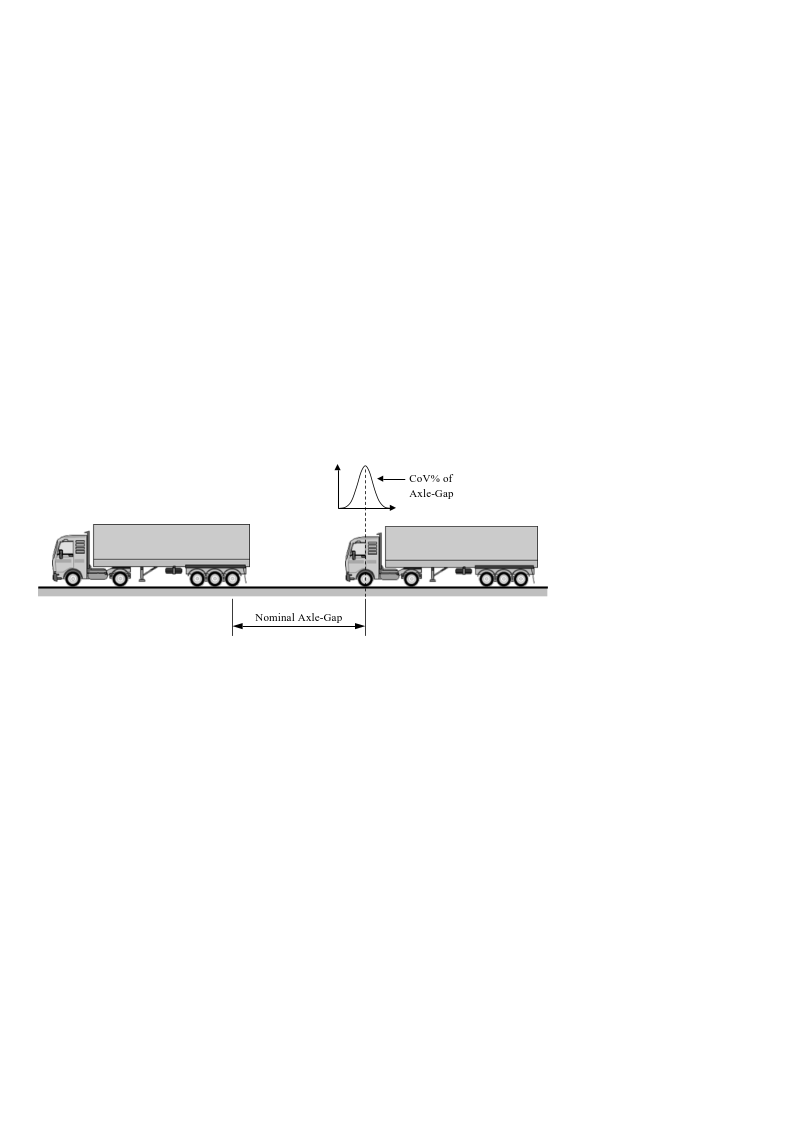
\includegraphics[width=5.34861in,height=2.04653in]{media/image5.png}

\begin{itemize}
\item
  ``6'' -- Free-flow model which uses a Poisson arrival assumption based
  upon the Normalized Headway Model of Crespo-Minguillón and Casas
  (1997). This accounts for different flow rates (\emph{Q}) as follows:
\end{itemize}

\[ F(t) = 1 - \mathrm{e}^{-\lambda t} \]

\begin{quote}
Where
$1/\lambda$
is the mean headway, i.e. the average time gap between vehicles in the
hour of the current total (cars and trucks) flowrate \emph{Q} and so is
given by \emph{Q}/3600.
\end{quote}

For all models the program checks that no overlapping of vehicles can
occur by ensuring the generated gap is greater than the required minimum
gap (taking account of the maximum bridge length, vehicle lengths, and
speed difference between them).

\paragraph*{Line 8:}\label{line-8}
\addcontentsline{toc}{paragraph}{Line 8:}

The traffic classification scheme to be used in output:

\begin{itemize}
\item
  0 -- classify by the number of axles
\item
  1 -- classify by the axle pattern, where axle groups are identified as
  consecutive axles with spacing \textless{} 2.1~m.
\end{itemize}

\paragraph*{Line 9:}\label{line-9}
\addcontentsline{toc}{paragraph}{Line 9:}

Specify the name of the Lane Flow definition file that is in the working
folder.

\paragraph*{Line 10:}\label{line-10}
\addcontentsline{toc}{paragraph}{Line 10:}

Specify the nominal axle gap for Headway Model 5 -- congestion.

\paragraph*{Line 11:}\label{line-11}
\addcontentsline{toc}{paragraph}{Line 11:}

Specify the speed of all vehicles for Headway Model 5 -- congestion.
Note that this, combined with the calculation time step (Line 16),
effectively renders a distance-stepping algorithm and so this speed can
be notional to achieve a required distance step.

\paragraph*{Line 12:}\label{line-12}
\addcontentsline{toc}{paragraph}{Line 12:}

Specify the coefficient of variation of the nominal congested gap for
Headway Model 5 -- congestion.

\paragraph*{Line 13:}\label{line-13}
\addcontentsline{toc}{paragraph}{Line 13:}

Specify the filename in the working folder for the garage of vehicles to
be used for Traffic Generation Model 2. Note, this file must be in the
format of the Traffic Input File specified in Line 16.

\paragraph*{\texorpdfstring{Line 14: }{Line 14: }}\label{line-14}
\addcontentsline{toc}{paragraph}{Line 14: }

Specify the filename in the working folder of the kernel specifications
for the Traffic Generation Model 2.

\paragraph*{Line 15:}\label{line-15}
\addcontentsline{toc}{paragraph}{Line 15:}

Specify the name of the traffic input file in the working folder for
Program Mode 3.

\paragraph*{Line 16:}\label{line-16}
\addcontentsline{toc}{paragraph}{Line 16:}

Specify the format of the input file: 1 -- CASTOR format, 2 -- BeDIT, 3
-- DITIS format, 4 -- MON, 5 -- SiWIM CSV (introduced in v1.3.7, input
only). See Appendix for traffic file format definitions.

\paragraph*{Line 17:}\label{line-17}
\addcontentsline{toc}{paragraph}{Line 17:}

BTLS normally passes each vehicle across the bridge according to its own
speed when in Program Mode 3. Setting this option to ``1'' imposes
constant speed on all vehicles for comparison with some other algorithms
-- mostly to do with congestion traffic files.

\paragraph*{Line 18:}\label{line-18}
\addcontentsline{toc}{paragraph}{Line 18:}

When constant speed is imposed (Line 11), if this option is ``1'' then
the average speed of all vehicles in the file will be used, otherwise
the speed specified in Line 19 will be used.

\paragraph*{Line 19:}\label{line-19}
\addcontentsline{toc}{paragraph}{Line 19:}

Specifies the constant speed if Line 17 is ``1'' and Line 18 is ``0''.

\paragraph*{Line 20:}\label{line-20}
\addcontentsline{toc}{paragraph}{Line 20:}

Specify the name of the bridge definition file (see Section 0) in the
working folder.

\paragraph*{Line 21:}\label{line-21}
\addcontentsline{toc}{paragraph}{Line 21:}

Specify the name of the influence line definition file (see Section 3.6)
in the working folder.

\paragraph*{Line 22:}\label{line-22}
\addcontentsline{toc}{paragraph}{Line 22:}

Specify the name of the influence surface definition file (see Section
3.7) in the working folder.

\paragraph*{Line 23:}\label{line-23}
\addcontentsline{toc}{paragraph}{Line 23:}

Specify the calculation time step which is used in passing the vehicles
over the bridges. 0.1 s has been found a good compromise between
accuracy and efficiency. For some very sharp influence lines (e.g. shear
forces) a finer step may be required. A sensitivity study is
recommended.

\paragraph*{Line 24:}\label{line-24}
\addcontentsline{toc}{paragraph}{Line 24:}

To avoid unnecessary computation of smaller vehicles, this specifies the
minim GVW for a vehicle's load effect to be calculated. Its spatial
arrangement on the road is not affected if its GVW is less than this
number. The units are deci-tonnes (t/10)

\paragraph*{Line 25:}\label{line-25}
\addcontentsline{toc}{paragraph}{Line 25:}

Specify ``1'' to write a full time history of the load effects -- see
section on BTLS Output for more details. This should be set to ``0'' for
long simulations due to enormous resulting file size and slow execution.

\paragraph*{Line 26:}\label{line-26}
\addcontentsline{toc}{paragraph}{Line 26:}

Specify ``1'' to write the load effect value for each loading event that
occurs. Again this can be a large file and cause slow execution for
long-run simulations. See section on BTLS Output for more details.

\paragraph*{Line 27:}\label{line-27}
\addcontentsline{toc}{paragraph}{Line 27:}

If each loading event value is to be written (Line 24), this option if
set to ``1'' specifies the number of events that are stored in memory
before writing to the hard drive. See section on BTLS Output for more
details (Section 5).

\paragraph*{Line 28:}\label{line-28}
\addcontentsline{toc}{paragraph}{Line 28:}

Writes a file suitable for further fatigue calculations, giving load
cycles.

\paragraph*{\texorpdfstring{Line 29: }{Line 29: }}\label{line-29}
\addcontentsline{toc}{paragraph}{Line 29: }

Conduct Rainflow analysis on the load effects, which is for fatigue
research.

\paragraph*{\texorpdfstring{Line 30: }{Line 30: }}\label{line-30}
\addcontentsline{toc}{paragraph}{Line 30: }

The number of decimals kept for Rainflow analysis, acting as the bin
size.

\paragraph*{\texorpdfstring{Line 31: }{Line 31: }}\label{line-31}
\addcontentsline{toc}{paragraph}{Line 31: }

The cutoff value for Rainflow analysis.

\paragraph*{\texorpdfstring{Line 32: }{Line 32: }}\label{line-32}
\addcontentsline{toc}{paragraph}{Line 32: }

Rainflow-output file buffer size.

\paragraph*{Line 33:}\label{line-33}
\addcontentsline{toc}{paragraph}{Line 33:}

For all program modes, this option if ``1'' will write the generated or
read-in vehicle file. For long run simulations this should be ``0'' as
very large files can result, filling hard drive space and causing very
slow computation. Mostly useful for short debugging or test runs.

\paragraph*{Line 34:}\label{line-34}
\addcontentsline{toc}{paragraph}{Line 34:}

This specifies the format of the output file traffic file: 1 -- CASTOR
format, 2 -- BeDIT, 3 -- DITIS, 4 -- MON. Note that the SiWIM CSV
format (5) is read-only and cannot be used for output.

\paragraph*{Line 35:}\label{line-35}
\addcontentsline{toc}{paragraph}{Line 35:}

The name of the file to be written if Line 33 is ``1''.

\paragraph*{Line 36:}\label{line-36}
\addcontentsline{toc}{paragraph}{Line 36:}

If the vehicle file is to be written (Line 33 set to ``1''), this
specifies the number of vehicles that are stored in memory before
writing to the hard drive. See section on BTLS Output for more details.

\paragraph*{Line 37:}\label{line-37}
\addcontentsline{toc}{paragraph}{Line 37:}

If this is set to ``1'' files are output giving the traffic flow and
composition information for each hour of the simulation for each lane.

\paragraph*{Line 38:}\label{line-38}
\addcontentsline{toc}{paragraph}{Line 38:}

If this option is ``1'' calculations are performed that can be used to
write block maxima output. Set to ``0'' to override all block maxima
output and calculations.

\paragraph*{Line 39:}\label{line-39}
\addcontentsline{toc}{paragraph}{Line 39:}

For block maximum output, this specifies the block size in days for
which the maximum is retained (it can be zero if Line 40 has a number
\textgreater{} 0).

\paragraph*{Line 40:}\label{line-40}
\addcontentsline{toc}{paragraph}{Line 40:}

For block maximum output, this specifies the block size in seconds for
which the maximum is retained (it can be zero if Line 39 has a number
\textgreater{} 0).

\paragraph*{Line 41:}\label{line-41}
\addcontentsline{toc}{paragraph}{Line 41:}

Specify ``1'' to write block maximum load effect and vehicle output
files for each number of vehicles comprising the events. See section on
BTLS Output (Section 5.4) for more details.

\paragraph*{Line 42:}\label{line-42}
\addcontentsline{toc}{paragraph}{Line 42:}

Specify whether to write the block maximum summary files (``1'' or
``0''). See section on BTLS Output (Section 5.4) for more details.

\paragraph*{Line 43:}\label{line-43}
\addcontentsline{toc}{paragraph}{Line 43:}

Specify ``1'' to write block maximum load effect output files for which
the events are not separated by the number of vehicles in the event, or
``0'' to not. See section on BTLS Output (Section 5.4) for more details.

\paragraph*{Line 44:}\label{line-44}
\addcontentsline{toc}{paragraph}{Line 44:}

If block maximum output is to be written (Line 38), this option if set
to ``1'' specifies the number of events that are stored in memory before
writing to the hard drive. See section on BTLS Output (Section 5.4) for
more details.

\paragraph*{Line 45:}\label{line-45}
\addcontentsline{toc}{paragraph}{Line 45:}

If this option is ``1'' calculations are performed that can be used to
write peaks-over-threshold (POT) output. Set to ``0'' to override all
POT output and calculations. Note that the thresholds for each load
effect are set in the Bridge Definition File (Section 0).

\paragraph*{Line 46:}\label{line-46}
\addcontentsline{toc}{paragraph}{Line 46:}

For POT output, this specifies if the vehicles comprising the peak
events are to be output to a vehicle-event file. See section on BTLS
Output (Section 5.5) for more details.

\paragraph*{Line 47:}\label{line-47}
\addcontentsline{toc}{paragraph}{Line 47:}

For POT output, this specifies if summary files are to be written. See
section on BTLS Output (Section 5.5) for more details.

\paragraph*{Line 48:}\label{line-48}
\addcontentsline{toc}{paragraph}{Line 48:}

For POT output, this specifies if a peaks counter file is to be written.
See section on BTLS Output (Section 5.5) for more details.

\paragraph*{Line 49:}\label{line-49}
\addcontentsline{toc}{paragraph}{Line 49:}

For peaks counter output, this specifies the interval size in days for
which the peaks are counted (it can be zero if Line 50 has a number
\textgreater{} 0).

\paragraph*{Line 50:}\label{line-50}
\addcontentsline{toc}{paragraph}{Line 50:}

For peaks counter output, this specifies the interval size in seconds
for which the peaks are counted (it can be zero if Line 49 has a number
\textgreater{} 0).

\paragraph*{Line 51:}\label{line-51}
\addcontentsline{toc}{paragraph}{Line 51:}

If POT output is to be written (Line 41), this option if set to ``1''
specifies the number of events that are stored in memory before writing
to the hard drive. See section on BTLS Output (Section 5.5) for more
details.

\paragraph*{Line 52:}\label{line-52}
\addcontentsline{toc}{paragraph}{Line 52:}

If this option is ``1'' calculations are performed that accumulate
simple statistics of load effect and vehicles throughout the simulation.
Set to ``0'' to override all statistics output and calculations.

\paragraph*{Line 53:}\label{line-53}
\addcontentsline{toc}{paragraph}{Line 53:}

This specifies if the statistics for each load effect accumulated
through the whole simulation are to be output. See section on BTLS
Output (Section 5.6) for more details.

\paragraph*{Line 54:}\label{line-54}
\addcontentsline{toc}{paragraph}{Line 54:}

This specifies if the statistics for each load effect are to be output
at particular time intervals. See section on BTLS Output (Section 5.6)
for more details.

\paragraph*{Line 55:}\label{line-55}
\addcontentsline{toc}{paragraph}{Line 55:}

If interval statistics are to be output, this specifies the interval
duration. See section on BTLS Output (Section 5.6) for more details.

\paragraph*{Line 56:}\label{line-56}
\addcontentsline{toc}{paragraph}{Line 56:}

If interval statistics are to be output, this specifies the number of
intervals that are stored in memory before writing to file.

\subsection{Bridge Definition File}\label{bridge-definition-file}

The bridges over which vehicles are to pass are defined in the bridge
definition file, specified in the configuration file (BTLSin.txt). The
file name is arbitrary.

\textbf{\ul{Important!}}

A bridge definition file must be included in the working folder.

An example bridge definition file for a single bridge with 4 load
effects is shown:

\begin{longtable}[]{@{}
  >{\centering\arraybackslash}p{(\linewidth - 2\tabcolsep) * \real{0.1556}}
  >{\raggedright\arraybackslash}p{(\linewidth - 2\tabcolsep) * \real{0.8444}}@{}}
\toprule\noalign{}
\begin{minipage}[b]{\linewidth}\centering
Line No.
\end{minipage} & \begin{minipage}[b]{\linewidth}\raggedright
File
\end{minipage} \\
\midrule\noalign{}
\endhead
\bottomrule\noalign{}
\endlastfoot
1

2

3

4

5

6

7

8

9

10 & 1, 40.0, 2, 4

1, 1, 3000.0

1, 1, 0.728125, 0.271875

2, 1, 3000.0

2, 1, 0.728125, 0.271875

3, 2, 3000.0

2, 2, 0.728125

2, 2, 0.271875

4, 3, 3000.0

1 \\
\end{longtable}

Any number of bridges can be defined, as can any number of load effects
for each bridge. Each bridge definition is formatted as follows:

\paragraph*{Bridge Information: (e.g. ``1, 40.0, 2,
4'')}\label{bridge-information-e.g.-1-40.0-2-4}
\addcontentsline{toc}{paragraph}{Bridge Information: (e.g. ``1, 40.0, 2,
4'')}

This first line specifies some general information about the bridge:

\begin{itemize}
\item
  Column 1: the bridge number, a positive integer -- 1 in this case;
\item
  Column 2: the span of the bridge in metres, a real positive number --
  40.0 m in this case;
\item
  Column 3: the number of lanes on the bridge, a positive integer -- 2
  in this case;
\item
  Column 4: the number of load effects to be considered for this bridge,
  a positive integer -- 4 in this case.
\end{itemize}

Each load effect is then defined on the following lines with a format
depending on the type of load effect. The first line in each case is the
basic information, formatted as follows:

\paragraph*{Load Effect Information: (e.g. ``1, 1,
3000.0'')}\label{load-effect-information-e.g.-1-1-3000.0}
\addcontentsline{toc}{paragraph}{Load Effect Information: (e.g. ``1, 1,
3000.0'')}

\begin{itemize}
\item
  Field 1: the load effect number, a positive integer -- e.g. 1.
\item
  Field 2: the load effect definition type:

  \begin{itemize}
  \item
    1 -- lane factors are applied to a single influence line;
  \item
    2 -- separate influence lines and lane weights are applied to each
    lane;
  \item
    3 -- an influence surface is used for the load effect.
  \end{itemize}
\item
  Field 3: the threshold to be used for this load effect in
  peaks-over-threshold analysis, e.g. 3000.0 kNm. If this number is
  absent it is assumed to be zero.
\end{itemize}

The line(s) following the load effect information line are formatted
differently depending on the load effect definition type, 1, 2, or 3, as
follows:

\textbf{Load Effect Definition Type 1 -- Lane factors applied to single
IL}

Only one line is required in this case, for example ``1, 1, 0.728125,
0.271875'' (line 3) in the file above. This line is formatted as
follows:

\begin{itemize}
\item
  Field 1: The type of influence line:

  \begin{itemize}
  \item
    1 -- if it is a built-in influence line;
  \item
    2 -- if it is a user-defined discrete influence line.
  \end{itemize}
\item
  Field 2: The influence line number (whether built-in or discrete).
\item
  Fields3+: the lane factors to be applied to the influence line for
  Lane 1, 2 etc.
\end{itemize}

Line 5 in the file above shows that a discrete influence line is being
used for Load Effect 2 with lane factors for all lanes.

\textbf{Load Effect Definition Type 2 -- Separate ILs and lane weights
for each lane}

In this case a line is required, corresponding to each lane, formatted
as follows:

\begin{itemize}
\item
  Field 1: The type of influence line:

  \begin{itemize}
  \item
    1 -- if it is a built-in influence line;
  \item
    2 -- if it is a user-defined discrete influence line.
  \end{itemize}
\item
  Field 2: The influence line number (whether built-in or discrete).
\item
  Fields3: the lane factor to be applied to the influence line for this
  lane.
\end{itemize}

In the example file above, load effect 3, starting on line 6, is using
this form of definition. Line 7 defines that Lane 1 uses discrete IL
number 2 with lane weight 0.728125. Similarly, line 8 defines that Lane
2 uses the same discrete IL number 2 with lane weight 0.271875.

\textbf{Load Effect Definition Type 3 -- An influence surface is used
for the bridge}

In this case only a single line is required, assigning an influence
surface number to the load effect. Thus, in the above file, line 9 shows
that load effect 4 is using an influence surface, whilst line 10 assigns
influence surface 1 to it.

Lane factors represent the proportion of load of the corresponding lane
(i.e. lane factor 3 is for lane 3) that contributes to the load effect
in the element under consideration. In this way, an influence surface is
effectively defined as slices along each lane. Note that this model
means that the influence surface must be a scaled version of itself
transversely across the bridge -- this is not always the case however.

Finally, it can be noted that the above example file is a test file: all
of the load effects use different means of arriving at the same outcome
once the discrete influence line is for mid-span bending moment, and the
influence surface is that given as the example influence surface later
on.

\subsubsection*{\texorpdfstring{\hfill\break
Built-In Influence
Functions}{ Built-In Influence Functions}}\label{built-in-influence-functions}
\addcontentsline{toc}{subsubsection}{\hfill\break
Built-In Influence Functions}

The built-in influence functions are mathematical expressions that apply
for any bridge length and can be weighted with any value of lane factor.
Consequently, these built-in functions execute more quickly than read-in
influence lines.

The description and index for the built in functions are:

\begin{longtable}[]{@{}
  >{\raggedright\arraybackslash}p{(\linewidth - 4\tabcolsep) * \real{0.1406}}
  >{\raggedright\arraybackslash}p{(\linewidth - 4\tabcolsep) * \real{0.7271}}
  >{\centering\arraybackslash}p{(\linewidth - 4\tabcolsep) * \real{0.1323}}@{}}
\toprule\noalign{}
\begin{minipage}[b]{\linewidth}\raggedright
\textbf{Index}
\end{minipage} & \begin{minipage}[b]{\linewidth}\raggedright
\textbf{Influence Line}
\end{minipage} & \begin{minipage}[b]{\linewidth}\raggedright
\textbf{Location}
\end{minipage} \\
\midrule\noalign{}
\endhead
\bottomrule\noalign{}
\endlastfoot
1 & Mid-span bending moment for a simply supported beam & B \\
2 & Bending moment over the central support of a two-span beam & E \\
3 & Left-hand shear in a simply-supported beam & A \\
4 & Right-hand shear in a simply-supported beam & C \\
5 & Left-hand shear for a two-span beam & D \\
6 & Right-hand shear for a two-span beam & F \\
7 & Total amount of load on the bridge (i.e. the unit influence line)
& \\
8 & Bending moment at the 2\textsuperscript{nd} support of a three-span
beam & G \\
9 & Bending moment at the 3\textsuperscript{rd} support of a three-span
beam & H \\
\end{longtable}

A

B

C

D

E

F

G

~

000000000~

H

\subsection{Lane Flow Data File}\label{lane-flow-data-file}

This file contains all information relating to the number of lanes, the
flow in each lane throughout the day, and the traffic composition. It
applies when artificial traffic is being created using one of the
free-flow headway models.

\textbf{\ul{Important!}}

A lane flow definition file must be included in the working folder.

This file must be in *.csv format (but can have a *.txt extension). In
*.csv format it is easily edited in a spread sheet program as shown:

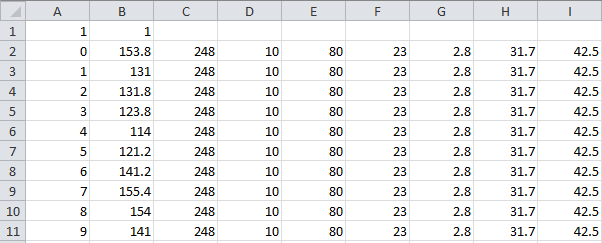
\includegraphics[width=6.26736in,height=2.53472in]{media/image8.png}

Each lane of the simulation is defined by 25 rows of data:

\begin{itemize}
\item
  The first row defines the lane number (sequential) and direction
  number (1 or 2) in columns 1 and 2 (or A and B in the screenshot);
\item
  The next 24 rows describe the traffic flow for each hour of the day
  (i.e. rows 2, 3, 4\ldots{} in the screenshot above).
\end{itemize}

Note that it is assumed that every day of the simulation is the same.
Typically only economic days of traffic are simulated of 5 days per
week, 50 weeks per year (250 days per year). It is assumed that each
such day has the same properties.

The structure of each hour description is as follows, with numbers given
from hour 0 of the screen shot above (at row 2):

\begin{itemize}
\item
  Column 1: The hour identifier, starting at midnight, 0 to 23 (e.g. 0)
\item
  Column 2: The mean truck flow rate in this hour (trucks/hour) (e.g.
  153.8)
\item
  Column 3: Mean velocity of traffic (dm/s) (e.g. 248)
\item
  Column 4: Standard deviation of the velocity (dm/s) (e.g. 10)
\item
  Column 5: Percentage of cars in this traffic model (e.g. 80)
\item
  Column 6: Percentage of trucks that are 2 axle (e.g. 23)
\item
  Column 7: Percentage of trucks that are 3 axles (e.g. 2.8)
\item
  Column 8: Percentage of trucks that are 4 axles (e.g. 31.7)
\item
  Column 9: Percentage of trucks that are 5 axles (e.g. 42.5)
\end{itemize}

The rationale for having the input in this form is the ease of altering
the percentage cars and overall flow rate without modifying the truck
flow and composition. This is best explained through an example of the
calculations the program performs:

\begin{enumerate}
\def\labelenumi{\arabic{enumi}.}
\item
  From Column 5, the truck percentage is 100-80 = 20\%;
\item
  This 20\% represents a flow of 153.8 vehicles per hour (Column2);
\item
  Thus the total flow rate is 153.8/0.2 = 769 vehicles per hour.
\item
  Of the 20\% vehicles that are trucks, for example, 42.5\% are 5-axle
  trucks, thus there will be 0.425*153.8 = 65.4 5-axle trucks on average
  for this hour.
\end{enumerate}

Changing Column 4 then changes the overall flow rate, without changing
the number of trucks that arrive.

Note that a normal distribution is assumed for the speed of all
vehicles.

Each lane to be included in the simulation must have the above
information. An example file with two lanes, one in each direction is
given below:

1,1,,,,,,,

0,153.8,248,10,80,23,2.8,31.7,42.5

1,131,248,10,80,23,2.8,31.7,42.5

2,131.8,248,10,80,23,2.8,31.7,42.5

3,123.8,248,10,80,23,2.8,31.7,42.5

4,114,248,10,80,23,2.8,31.7,42.5

5,121.2,248,10,80,23,2.8,31.7,42.5

6,141.2,248,10,80,23,2.8,31.7,42.5

7,155.4,248,10,80,23,2.8,31.7,42.5

8,154,248,10,80,23,2.8,31.7,42.5

9,141,248,10,80,23,2.8,31.7,42.5

10,126.4,248,10,80,23,2.8,31.7,42.5

11,101.6,248,10,80,23,2.8,31.7,42.5

12,95.8,248,10,80,23,2.8,31.7,42.5

13,88.2,248,10,80,23,2.8,31.7,42.5

14,93,248,10,80,23,2.8,31.7,42.5

15,109,248,10,80,23,2.8,31.7,42.5

16,124.2,248,10,80,23,2.8,31.7,42.5

17,151,248,10,80,23,2.8,31.7,42.5

18,141.8,248,10,80,23,2.8,31.7,42.5

19,172.2,248,10,80,23,2.8,31.7,42.5

20,141.4,248,10,80,23,2.8,31.7,42.5

21,148,248,10,80,23,2.8,31.7,42.5

22,157.2,248,10,80,23,2.8,31.7,42.5

23,159.4,248,10,80,23,2.8,31.7,42.5

2,2,,,,,,,

0,92.2,222,10,80,21.9,2.3,31,44.8

1,79.6,222,10,80,21.9,2.3,31,44.8

2,67,222,10,80,21.9,2.3,31,44.8

3,74.8,222,10,80,21.9,2.3,31,44.8

4,81.6,222,10,80,21.9,2.3,31,44.8

5,94.8,222,10,80,21.9,2.3,31,44.8

6,102.4,222,10,80,21.9,2.3,31,44.8

7,121.2,222,10,80,21.9,2.3,31,44.8

8,127.4,222,10,80,21.9,2.3,31,44.8

9,127.2,222,10,80,21.9,2.3,31,44.8

10,112.2,222,10,80,21.9,2.3,31,44.8

11,111.4,222,10,80,21.9,2.3,31,44.8

12,110.2,222,10,80,21.9,2.3,31,44.8

13,146,222,10,80,21.9,2.3,31,44.8

14,160.4,222,10,80,21.9,2.3,31,44.8

15,152,222,10,80,21.9,2.3,31,44.8

16,151,222,10,80,21.9,2.3,31,44.8

17,167.2,222,10,80,21.9,2.3,31,44.8

18,179.6,222,10,80,21.9,2.3,31,44.8

19,164.8,222,10,80,21.9,2.3,31,44.8

20,206.6,222,10,80,21.9,2.3,31,44.8

21,228.4,222,10,80,21.9,2.3,31,44.8

22,189,222,10,80,21.9,2.3,31,44.8

23,138.8,222,10,80,21.9,2.3,31,44.8

\subsection{Influence Line Definition
File}\label{influence-line-definition-file}

This file stores the definitions of any discrete influence lines that
are required. It must be in *.csv format (but can have a *.txt
extension).

\textbf{\ul{Important!}}

\begin{quote}
An influence line definition file must be included in the working folder
if it is required for the analysis.
\end{quote}

The first line of the file is the number of influence lines defined
within. Subsequently, each influence line is defined with the following
structure:

\begin{itemize}
\item
  A first line giving the influence line number (Column 1) and the
  number of points defining the influence line (Column 2);
\item
  Subsequent lines define the influence line using \emph{x}, \emph{y},
  pairs for the location and ordinate values (Columns 1 and 2
  respectively).
\end{itemize}

Discrete influence line processing takes longer than built-in
expressions. The program must search the vector of \emph{x}-coordinates
to find the points surrounding the axle location. Linear interpolation
of the ordinates is then used to find the ordinate at the axle location.
The spacing of points need not be uniform. Therefore, prefer to use as
few points as is necessary where the influence line is linear, and more
points where it is curved.

\textbf{\ul{Important!}}

\begin{quote}
The program warns if the last \emph{x}-coordinate is not the same as the
length of the bridge defined in the Bridge Definition file. Behaviour in
this case is generally unpredictable. However this warning can be issued
due solely to rounding, and in this case no problems have been observed.
\end{quote}

An example file is given below:

\begin{itemize}
\item
  he first influence line is a test of a 40 m simply-supported mid-span
  bending moment calculation,
\item
  the second is an influence line from the Millau viaduct, courtesy if
  IFSTTAR, France.
\end{itemize}

2

1, 13

0.000000, 0.000000

3.333333, 4.695709

6.666667, 9.391137

10.000000, 14.086847

13.333333, 18.782556

16.666667, 23.477984

20.000000, 28.173693

23.333333, 23.477984

26.666667, 18.782556

30.000000, 14.086847

33.333333, 9.391137

36.666667, 4.695709

40.000000, 0.000000

2, 67

0.000000, 0.000000

3.200000, -1.404704

6.400000, -2.482683

9.600000, -2.967398

12.800000, -2.765344

16.000000, -1.658346

19.200000, 0.578218

22.400000, 4.170048

25.600000, 9.341767

28.800000, 16.319074

32.000000, 25.326593

35.200000, 36.574975

38.400000, 50.127631

41.600000, 31.722458

44.800000, 15.056238

48.000000, 0.000000

51.333333, -13.793401

54.666667, -25.918783

58.000000, -36.084887

61.333333, -44.196060

64.666667, -49.871840

68.000000, -52.900498

71.333333, -53.815114

74.666667, -52.833863

78.000000, -50.155575

81.333333, -46.221973

84.666667, -41.193196

88.000000, -35.436810

91.333333, -29.230102

94.666667, -22.847134

98.000000, -16.583464

101.333333, -10.646519

104.666667, -5.083589

108.000000, 0.000000

111.333333, 4.397896

114.666667, 8.216499

118.000000, 11.460109

121.333333, 14.100781

124.666667, 15.951508

128.000000, 16.941357

131.333333, 17.243363

134.666667, 16.930610

138.000000, 16.067582

141.333333, 14.799371

144.666667, 13.179716

148.000000, 11.327914

151.333333, 9.335319

154.666667, 7.293285

158.000000, 5.293167

161.333333, 3.385477

164.666667, 1.617506

168.000000, 0.000000

171.200000, -1.360639

174.400000, -2.545019

177.600000, -3.539167

180.800000, -4.268925

184.000000, -4.746116

187.200000, -4.978264

190.400000, -4.989011

193.600000, -4.803078

196.800000, -4.444110

200.000000, -3.936826

203.200000, -3.307020

206.400000, -2.577262

209.600000, -1.773345

212.800000, -0.904943

216.000000, 0.000000

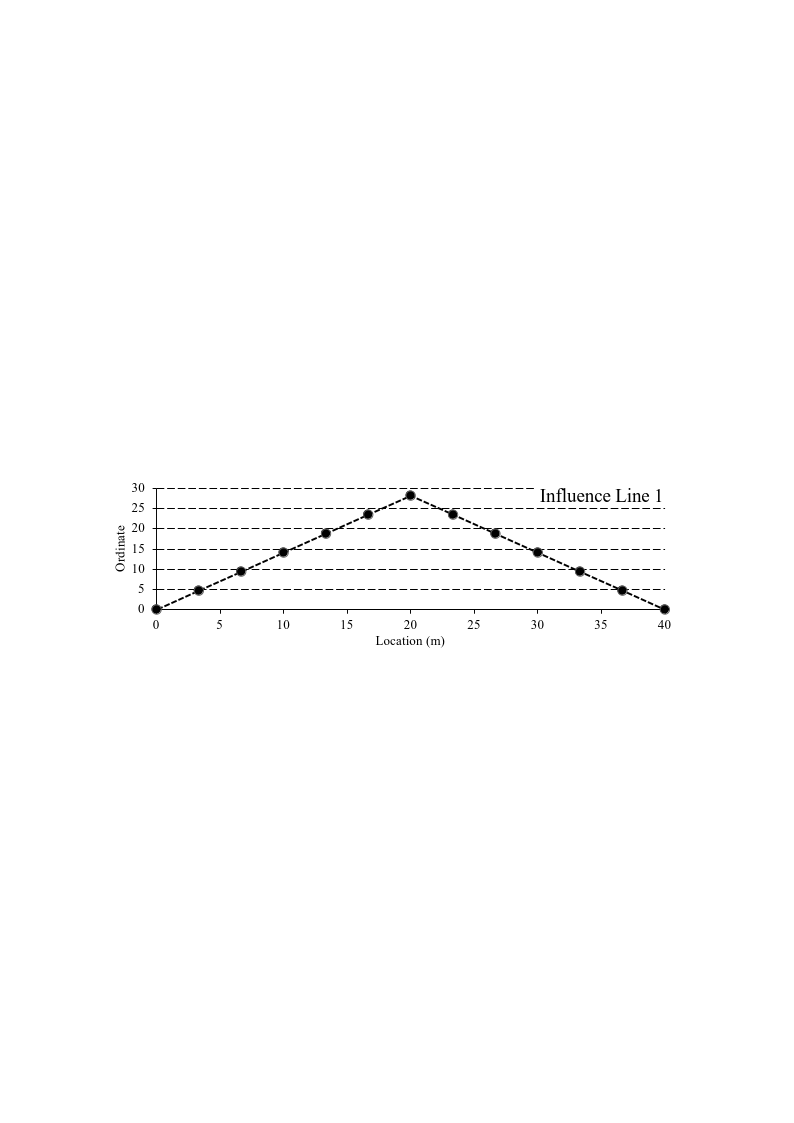
\includegraphics[width=6.02292in,height=1.84861in]{media/image9.png}

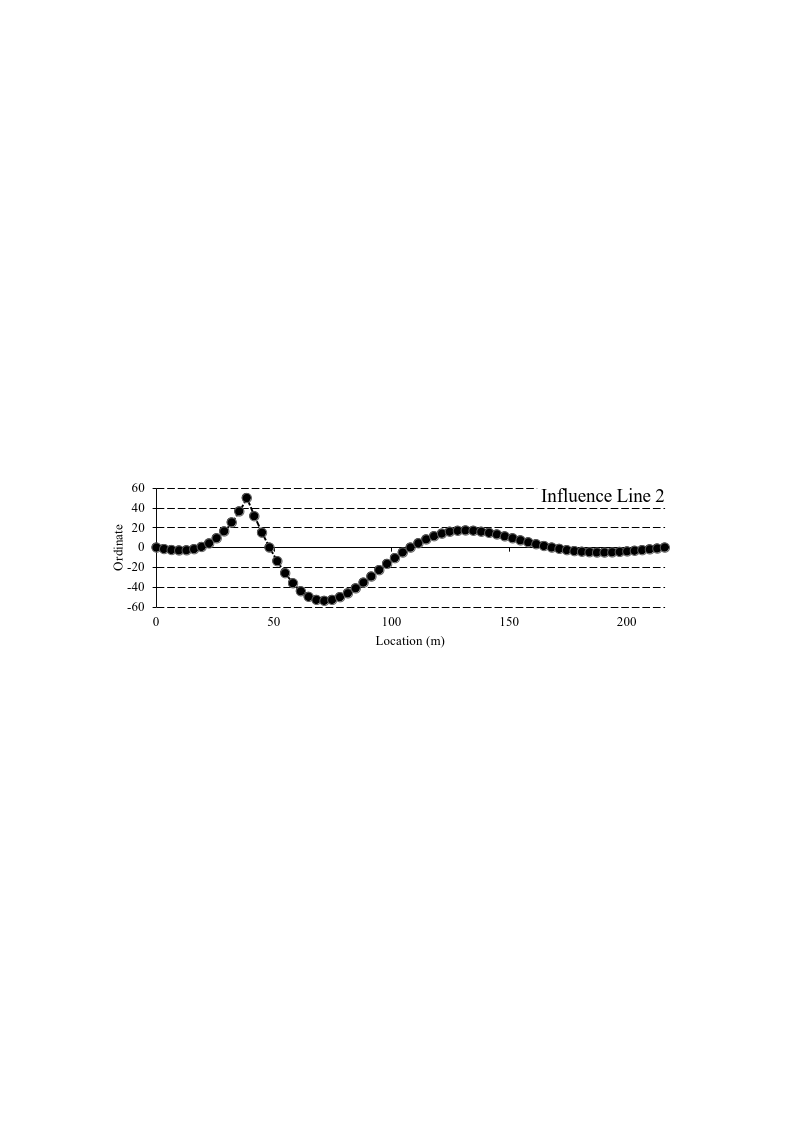
\includegraphics[width=6.02292in,height=1.84861in]{media/image10.png}

\subsection{Influence Surface Definition
File}\label{influence-surface-definition-file}

This file stores the definitions of any influence surfaces that are
required. It must be in *.csv format (but can have a *.txt extension).

\textbf{\ul{Important!}}

\begin{quote}
An influence surface definition file must be included in the working
folder if it is required for the analysis.
\end{quote}

Any number of influence surfaces can be defined in the file. Each
influence surface is defined on a rectangular grid according to a
specific format as follows:

\begin{itemize}
\item
  The first line defines the basic data as follows:

  \begin{itemize}
  \item
    Field 1: the influence surface number;
  \item
    Field 2: the number of rows of data (the number of \emph{x}- or
    longitudinal coordinates) specifying the influence surface grid
    points;
  \item
    Field 3: the number of lanes on the bridge/influence line
  \item
    Field 3+\emph{i}: the location of the edge of lane \emph{i} on the
    influence surface;
  \item
    Last Field: the upper edge of the last lane.
  \end{itemize}
\item
  Line 2 defines the \emph{y}- or transverse coordinates of the grid
  points.
\item
  Each row then defines the ordinates at the grid points, the first
  value of which is the \emph{x}-coordinate.
\end{itemize}

It is taken that Direction 1 traffic travels in the positive
\emph{x}-direction. For load application between grid points, linear
interpolation is used in both directions. Hence, for flat areas of the
influence surface a larger grid size can be used, but for more peaked
zones, a more refined grid is required.

An example file is shown below in which a single test influence surface
for mid-span bending moment of an edge beam is defined for comparison
with a standard method using built-in or discrete influence lines and
lane factors. The following figure describes the file and its
definitions.

1,5,2,0.35,4.0,7.65

0,0,2,4,6,8

0,0,0,0,0,0

10,5,3.75,2.5,1.25,0

20,10,7.5,5,2.5,0

30,5,3.75,2.5,1.25,0

40,0,0,0,0,0

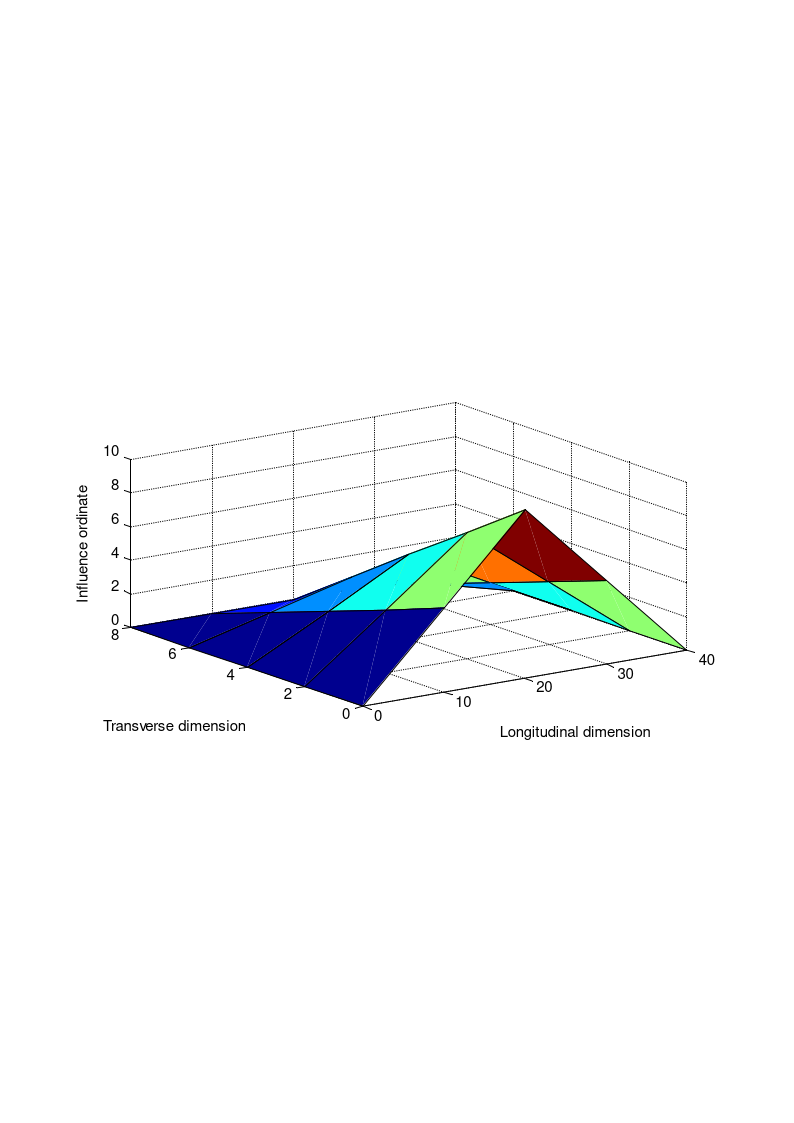
\includegraphics[width=4.9125in,height=2.55347in]{media/image11.png}

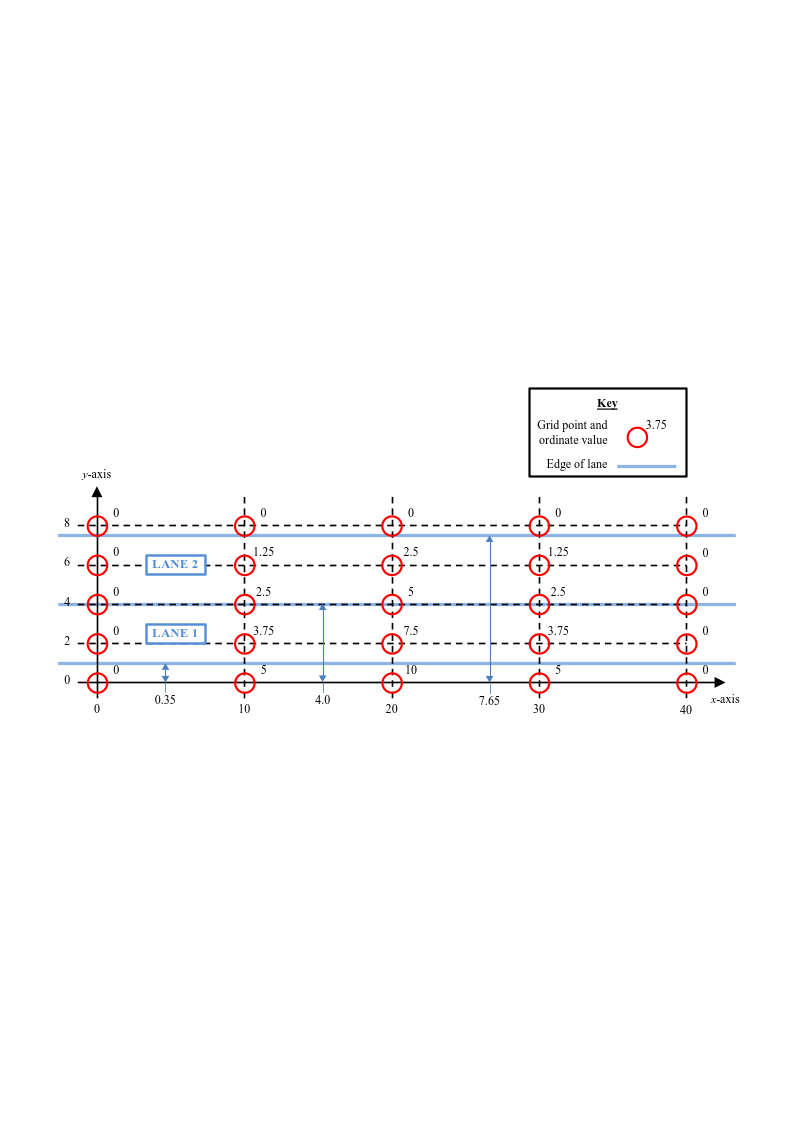
\includegraphics[width=6.68611in,height=3.40694in]{media/image12.png}

\textbf{\ul{Important!}}

\begin{quote}
If multiple influence surfaces are defined for a bridge, the program
assumes that the lane coordinates are the same for all influence
surfaces. This is as it should be for a single real bridge of course.
However, different lane coordinates can be used with different influence
surface definitions for different bridges under the same traffic, either
read or generated.
\end{quote}

\section{Using BTLS}\label{using-btls}

\subsection{Running the program}\label{running-the-program}

The program can be run from any folder as explained previously. An
example working folder showing all files necessary to execute the
program is given below:

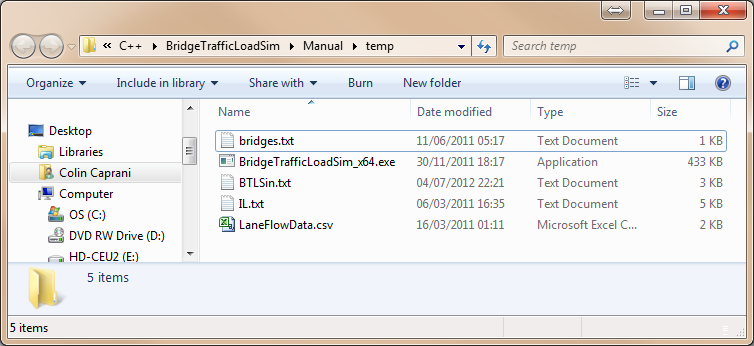
\includegraphics[width=6.5in,height=2.98819in]{media/image13.png}

Note that the 64 bit version is being used here.

\textbf{\ul{Important!}}

To run the program, double click the executable (*.exe) file on
Windows, or execute \texttt{./BTLS} from a terminal in the working
folder on Linux and macOS.

As of v1.3.7, if the configuration file \texttt{BTLSin.txt} cannot be
found in the working folder, the program prints

\begin{quote}
\texttt{***ERROR:\ BTLSin\ file\ could\ not\ be\ opened:\ BTLSin.txt}
\end{quote}

and exits immediately with a non-zero exit code. (Earlier versions
attempted to continue with built-in default values, which generally
led to a crash.) On success the program returns exit code 0, so BTLS
can be scripted reliably in batch runs.

\subsection{Console output}\label{console-output}

Some examples of console output during program execution are given.

\subsubsection*{Example 1: Program Mode
1}\label{example-1-program-mode-1}
\addcontentsline{toc}{subsubsection}{Example 1: Program Mode 1}

After each day of simulation is complete, the program outputs a notice.
At the end of the simulation the elapsed time is displayed for
information. In this case, 20 days of traffic and generated and
simulated crossing 5 bridges, each with 3 load effects.

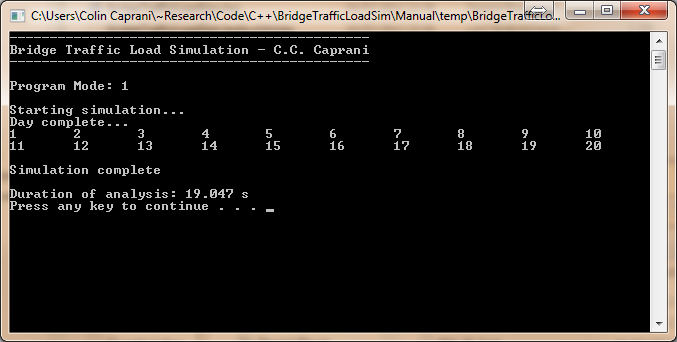
\includegraphics[width=6.5in,height=3.27917in]{media/image14.png}

\subsubsection*{\texorpdfstring{\hfill\break
Example 1: Program Mode
2}{ Example 1: Program Mode 2}}\label{example-1-program-mode-2}
\addcontentsline{toc}{subsubsection}{\hfill\break
Example 1: Program Mode 2}

Ten days of vehicles are generated and the current day number is given
(right hand columns). Each time the program flushed the vehicle buffer
to the file, an output is given of the simulation time at which it
occurred.

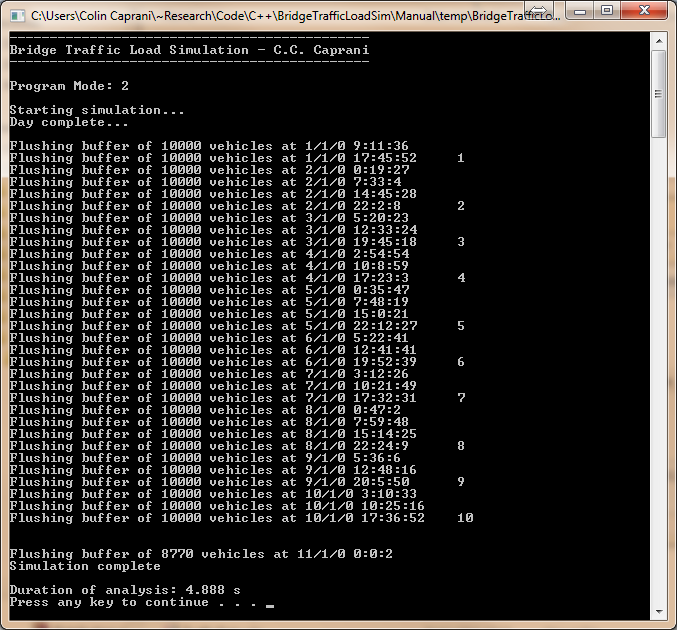
\includegraphics[width=6.5in,height=6.04653in]{media/image15.png}

The fodler is then populated with the outputted vehicle file as named in
``BTLSin.txt''.

\subsubsection*{\texorpdfstring{\hfill\break
Example 3: Program Mode
3}{ Example 3: Program Mode 3}}\label{example-3-program-mode-3}
\addcontentsline{toc}{subsubsection}{\hfill\break
Example 3: Program Mode 3}

The traffic file created in the last example is read in and passed over
5 bridges, each with 3 load effects. The output is as follows:

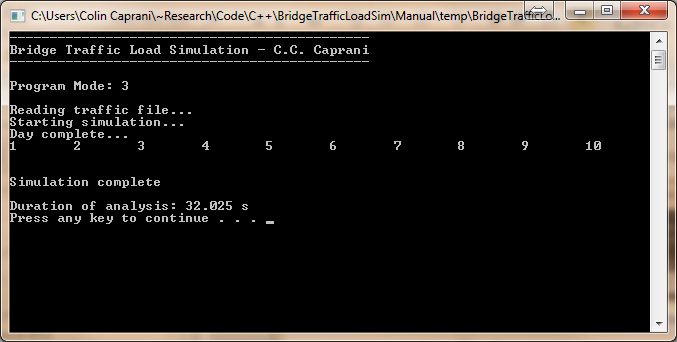
\includegraphics[width=6.5in,height=3.27917in]{media/image16.png}

Note the slower execution time than for Program Mode 1 which has 20 days
of traffic. This is caused by the additional overhead required to
manipulate the 25 MB traffic file that has been read into memory.

\subsection{Input Errors}\label{input-errors}

When there are errors in the input, the behaviour is unpredictable. More
informative user feedback will be built in soon.

Note that a missing \texttt{BTLSin.txt} is detected and reported
cleanly: the program exits with an error message and a non-zero exit
code (see Section 4.1).

Some potential problems:

\begin{itemize}
\item
  The supporting files (e.g. bridge, lane flow, IL) cannot be found in
  the working folder;
\item
  The traffic folder cannot be found (it should be at
  ``C:\textbackslash Traffic'');
\item
  The vehicle file to be read in cannot be found (Program Mode 3).
\item
  Outputs are not matched to Program Mode (e.g. Program Mode 2 --
  Generate vehicle file, but no vehicle file is to be output -- Line 20
  of BTLSin.txt.)
\end{itemize}

In each of these cases, the program may:

\begin{itemize}
\item
  Output helpful warnings;
\item
  Flash open and close immediately;
\item
  Remain open and display unusual text, such as ``Conversion Error''.
\end{itemize}

Admittedly, all behaviours should be of the first type -- this will
improve.

\section{BTLS Output}\label{btls-output}

\subsection{Introduction}\label{introduction-3}

BTLS can produce large amounts of output, especially for long run
simulations or heavily congested traffic. Accessing the hard drive often
can significantly slow the program's execution. Therefore, keep buffer
sizes as large as memory and execution speed can allow.

All outputs are in text file format with specific information layouts
and formats for each type of output file.

\subsubsection*{Effect on Execution
Speed}\label{effect-on-execution-speed}
\addcontentsline{toc}{subsubsection}{Effect on Execution Speed}

Obviously, the more outputs that are needed the slower the simulation.
Some general comments to aid execution time are:

\begin{itemize}
\item
  Only output what is needed: this can be ascertained by a few short
  runs before doing the main long-run simulation.
\item
  Use the buffer size variables to good effect: for sample runs monitor
  the program's RAM usage, increasing the buffer sizes as much as
  possible to prevent undue writing to disc, one of the slowest
  operations.
\item
  The statistics output is intended mainly for short runs to give
  information for peaks-over-threshold analysis (i.e. threshold levels).
  Consequently, turn it off when it is not required.
\item
  Similarly, the flow data output is only intended for short-run
  verification that the traffic is being properly modelled.
  Consequently, turn it off when it is not required.
\item
  For the Block Max and POT outputs, turn off the vehicle output files
  if they are not needed.
\end{itemize}

\subsection{Miscellaneous Output}\label{miscellaneous-output}

\subsubsection*{Time History File}\label{time-history-file}
\addcontentsline{toc}{subsubsection}{Time History File}

If a full time history is selected to be output (Line 25 of BTLSin.txt),
BTLS creates a single file for each bridge named:

TH\_L.txt

Where \emph{L} is the bridge length. The file gives the load effect at
each time step of the simulation for each load effect considered for the
bridge. Note that no output is given when there is zero load effect. A
sample output is:

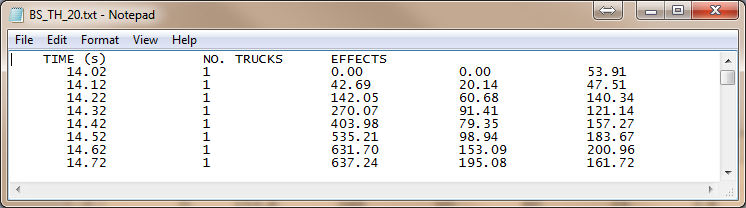
\includegraphics[width=6.5in,height=1.81389in]{media/image17.png}

The format is:

\begin{itemize}
\item
  Column 1: the current time. Note that time starts at the time of
  arrival of the first vehicle;
\item
  Column 2: The number of trucks currently on the bridge;
\item
  Columns 3+: The current value of each load effect is given, according
  to the order of the load effects in the bridge definition file.
\end{itemize}

This file can get extremely large, but for short runs (e.g. 1-day) it is
very useful for checking and debugging output.

An example output is given showing the number of trucks on the bridge
through the day. As can be seen, four 3-truck events occur on this 20 m
bridge.

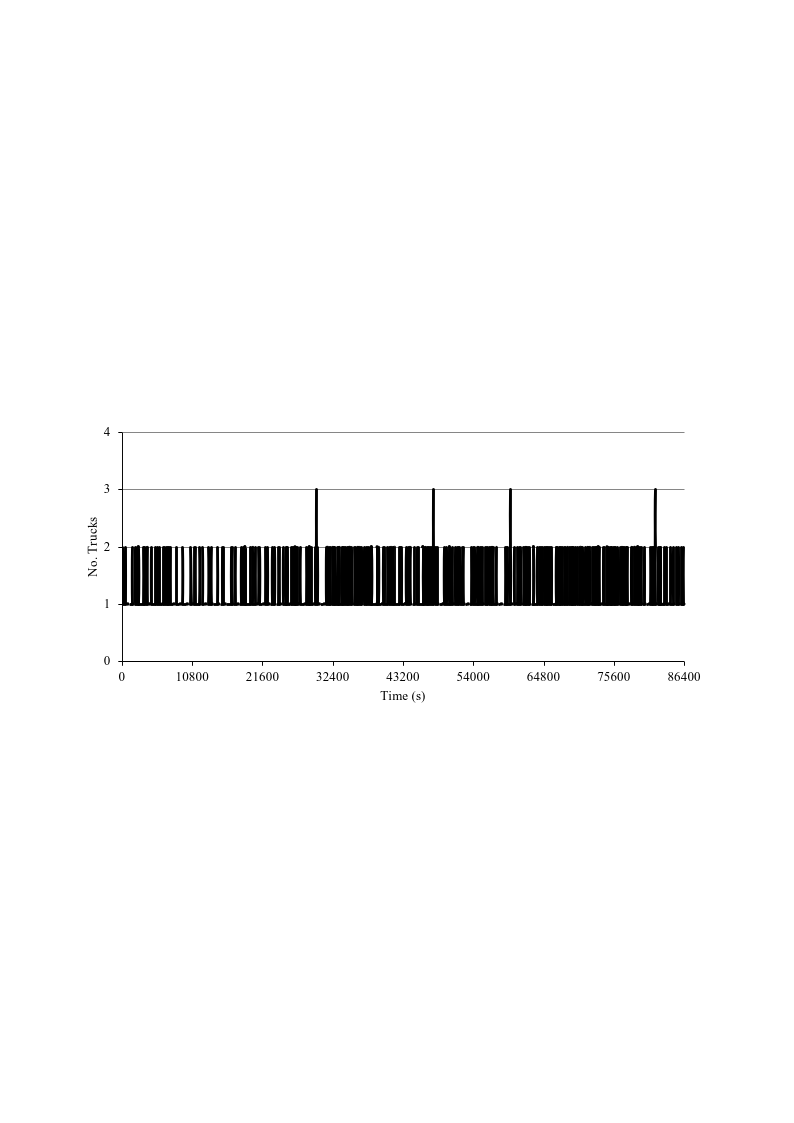
\includegraphics[width=6.63958in,height=3.01181in]{media/image18.png}

\subsubsection*{All Events File}\label{all-events-file}
\addcontentsline{toc}{subsubsection}{All Events File}

If all loading events are selected to be output (Line 26 of BTLSin.txt),
BTLS creates a single file for each bridge named:

BL\_L\_AllEvents.txt

Where \emph{L} is the bridge length. The file gives the maximum of each
calculated load effect recorded during each loading event to occur. A
loading event is defined as the loading that occurs between two
occasions of zero trucks on the bridge, or the departure or arrival of
another vehicle. A sample output is:

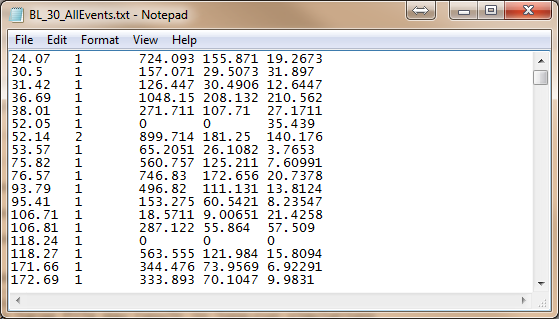
\includegraphics[width=5.19792in,height=2.96528in]{media/image19.png}

The format is:

\begin{itemize}
\item
  Column 1: the starting time of the loading event.
\item
  Column 2: The number of trucks in the event;
\item
  Columns 3+: The maximum value of each load effect during the event.
\end{itemize}

This file can get extremely large, but is useful for checking and
debugging output.

\subsubsection*{Fatigue Events File}\label{fatigue-events-file}
\addcontentsline{toc}{subsubsection}{Fatigue Events File}

If fatigue events are selected to be output (Line 28 of BTLSin.txt),
BTLS creates a single file for each bridge named:

BL\_L \_Fatigue.txt

Where \emph{L} is the bridge length. The file gives the maximum and
minimum values of each loading event (defined above) in chronological
order. This is suitable for examination of fatigue cycles. A sample
output is shown below:

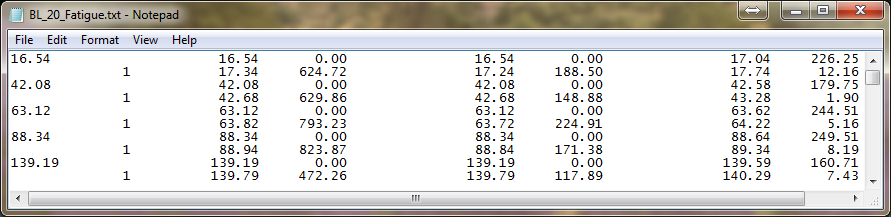
\includegraphics[width=6.5in,height=1.58125in]{media/image20.png}

The format is:

\begin{itemize}
\item
  Column 1 (Line 1): the starting time of the loading event;
\item
  Column 2 (Line 2): The number of trucks in the event.
\end{itemize}

For each line, the subsequent columns are:

\begin{itemize}
\item
  Column 3: The time at which the value of load effect 1 is recorded;
\item
  Column 4: the value of load effect 1.
\end{itemize}

Columns 5 \& 6 give the time and value of load effect 2, and so on.

For example, this file shows that load effect 3 had a maximum value at
17.04 s, followed by a minimum at 17.74 s.

\subsection{Vehicle Output}\label{vehicle-output}

\subsubsection*{Traffic File}\label{traffic-file}
\addcontentsline{toc}{subsubsection}{Traffic File}

A traffic file can be output in any Program Mode if selected on Line 29
of BTLSin.txt. For Program Mode 2, this must be selected.

The file is named as specified on Line 31 of BTLSin.txt.

The program outputs vehicles in CASTOR format. An example of the program
output for several trucks is given:

1001 1 1 2 0 12618155 54 43211 18 2743 27 0 0 0 0 0 0 0 0 0 0 0 0 0 0

1001 1 1 2 0 2 412133 137 67311 18 5441 6626 17 0 0 0 0 0 0 0 0 0 0 0 0

1001 1 1 2 0 2 598157 64 43211 18 3243 32 0 0 0 0 0 0 0 0 0 0 0 0 0 0

1001 1 1 2 0 44354134 336133511 18 7839 7040 6327 6327 63 0 0 0 0 0 0 0
0

1001 1 1 2 0 93062152 117 67311 18 3941 3926 39 0 0 0 0 0 0 0 0 0 0 0 0

1001 1 1 2 0101765131 97 44211 18 5344 44 0 0 0 0 0 0 0 0 0 0 0 0 0 0

\subsubsection*{Flow Statistics}\label{flow-statistics}
\addcontentsline{toc}{subsubsection}{Flow Statistics}

For generated or read-in vehicle files, selecting this option will
output files containing the flow rate and traffic stream composition.
The files are named:

FlowData\_D\_L.txt

Where \emph{D} is the direction number and \emph{L} is the lane number
corresponding to those in the Lane Flow Data definition file.

For each hour of the simulation, the following statistics are collected
for each lane:

\begin{itemize}
\item
  The number of vehicles in the hour
\item
  The number of trucks;
\item
  The number of cars;
\item
  The number of 2-axle, 3-axle, 4-axle and 5-axle trucks in the hour.
\end{itemize}

This output allows direct comparison with the input given in the Lane
Flow Definition file is generating traffic. A screenshot is shown below:

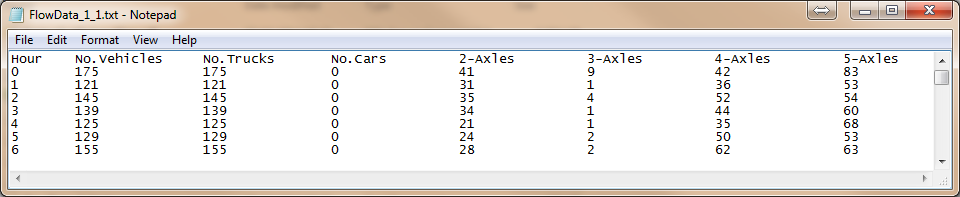
\includegraphics[width=6.5in,height=1.3375in]{media/image21.png}

\subsection{Block Maximum Files}\label{block-maximum-files}

If block maximum vehicle files are selected to be output (Line 34 of
BTLSin.txt), BTLS can creates different types of file output.

\subsubsection*{Output by Number of
Trucks}\label{output-by-number-of-trucks}
\addcontentsline{toc}{subsubsection}{Output by Number of Trucks}

This option is specified on Line 37 of BTLSin.txt. Output is given for
each load effect of each bridge named:

BM\_V\_L\_N.txt

Where \emph{L} is the bridge length and \emph{N} is the number of trucks
comprising the loading events. In this manner a comprehensive breakdown
of the causing of loading can be studied, suitable for application of
the CDS method (Caprani et al 2008).

A sample output is shown:

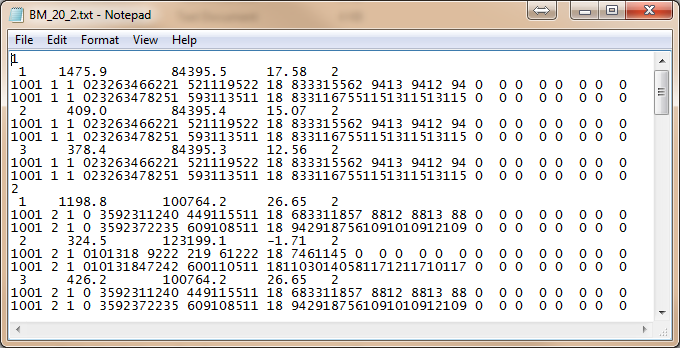
\includegraphics[width=6.5in,height=3.32569in]{media/image22.png}

This file structure is termed a Loading Event File, and its structure
explained later.

\subsubsection*{Summary Files}\label{summary-files}
\addcontentsline{toc}{subsubsection}{Summary Files}

If block maximum summary files are selected to be output (Line 38 of
BTLSin.txt), BTLS creates a file for each load effect of each bridge
named:

BM\_S\_L\_Eff\_E.txt

Where \emph{L} is the bridge length and \emph{E} is the load effect
number. The file gives the maximum load effect recorded during each
block, broken down according to the number of trucks comprising the
event. A sample output is:

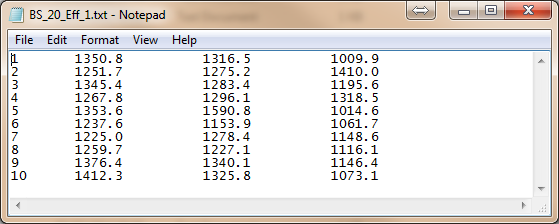
\includegraphics[width=5.82569in,height=2.3375in]{media/image23.png}

The format is:

\begin{itemize}
\item
  Column 1: The block index.
\item
  Column 2: The block maximum 1-truck load effect;
\item
  Columns 3: The block maximum 2-truck load effect
\item
  Columns 4+: As appropriate, the block maximum 3-, 4-, \ldots{} truck
  load effect.
\end{itemize}

Taking the maximum across Columns 2+ gives the overall block maximum
load effect.

\subsubsection*{Mixed Vehicle Output}\label{mixed-vehicle-output}
\addcontentsline{toc}{subsubsection}{Mixed Vehicle Output}

This option is specified on Line 39 of BTLSin.txt. This form of output
represents the conventional form in which the number of trucks
comprising the event is not taken into account. Instead, the maximum
load effect recorded during the block is noted. One such file per bridge
is output, named:

BM\_V\_L\_All.txt

Where \emph{L} is the bridge length. This file structure is a Loading
Event File, explained later. A sample output showing 3 blocks is:

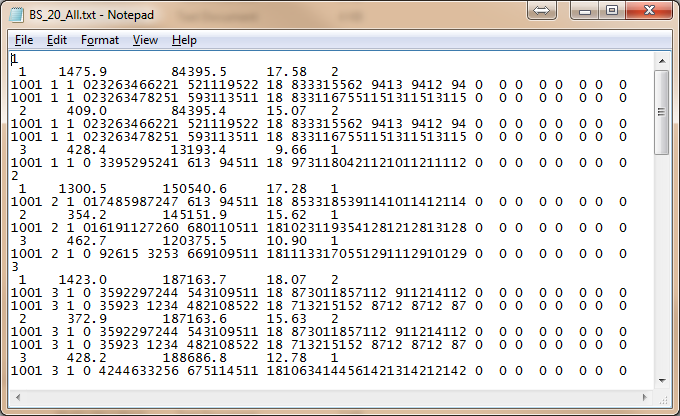
\includegraphics[width=5.75556in,height=3.52292in]{media/image24.png}

As can be seen, there are a different number of trucks comprising the
loading events that cause the maximum of each load effect in the block.
Sometimes the same truck(s) loading event causes the maximum of 2 or
more load effects, but in general different loading events cause the
maximum of each load effect. This is because of the different shapes of
the influence lines, and hence critical loading arrangements.

\subsection{Peaks-Over-Threshold
Files}\label{peaks-over-threshold-files}

If POT files are selected to be output (Line 41 of BTLSin.txt), BTLS can
creates two types of file output.

\subsubsection*{Vehicle Files}\label{vehicle-files}
\addcontentsline{toc}{subsubsection}{Vehicle Files}

This option is specified on Line 42 of BTLSin.txt. The vehicles
comprising the loading event that is a peak are output in a Loading
Event File structure. The files are named:

PT\_V\_L\_E.txt

Where \emph{L} is the bridge length and \emph{E} is the load effect
number. This file structure is a Loading Event File, explained later. A
sample output showing 2 peaks is:

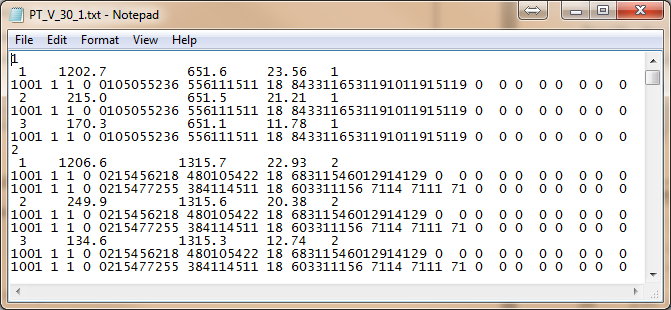
\includegraphics[width=6.5in,height=3in]{media/image25.png}

Note that the number of vehicles comprising the loading events are mixed
and not separated out.

\subsubsection*{Summary Files}\label{summary-files-1}
\addcontentsline{toc}{subsubsection}{Summary Files}

This option is specified on Line 43 of BTLSin.txt. The vehicles
comprising the loading event that is a peak are output in a Loading
Event File structure. The files are named:

PT\_S\_L\_Eff\_E.txt

Where \emph{L} is the bridge length and \emph{E} is the load effect
number. Each row of data in this file corresponds to a recorded peak.
For each peak, the following data is ouput:

\begin{itemize}
\item
  The peak number;
\item
  The time at which the peak occurred;
\item
  The number of truck sin the event;
\item
  The peak load effect value.
\end{itemize}

A screenshot of such a file is shown below.

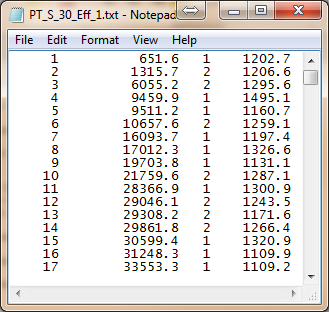
\includegraphics[width=3.10486in,height=2.94167in]{media/image26.png}

Note that since there is not much memory required to store peak
information, the buffer size defined on Line 36 of BTLSin.txt should be
large to prevent frequent disk writing which is slow.

\subsubsection*{Counter Files}\label{counter-files}
\addcontentsline{toc}{subsubsection}{Counter Files}

This option is specified on Line 44 of BTLSin.txt. The number of peaks
over the specified threshold occurring in each counter interval (defined
on Lines 45-6 of BTLSin.txt) is output for each load effect. The files
are named:

PT\_C\_L.txt

Where \emph{L} is the bridge length. Each row of data in this file
corresponds to a counter interval, and for each block and load effect
the number of peaks is given. A screenshot of such a file is shown
below.

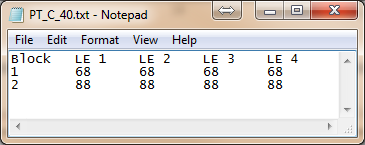
\includegraphics[width=3.80208in,height=1.51181in]{media/image27.png}

If the POT output buffer size (Line 47 of BTLSin.txt) is such that an
output occurs during a counter interval, then the interval will have two
rows (the number of peaks before output, and number after output) and
the total number of peaks will be the sum of the two results. Again,
since there is not much memory required to store peak information, the
buffer size defined on should be large to prevent frequent disk writing
which is slow.

\subsection{Load Effect Statistics
Output}\label{load-effect-statistics-output}

BTLS can output some useful summary statistics of the calculated load
effects. The statistics currently supported are:

\begin{itemize}
\item
  Events count;
\item
  The number of vehicles recorded;
\item
  The number of trucks recorded
\item
  The minimum load effect value;
\item
  The maximum load effect value;
\item
  The mean load effect value;
\item
  The standard deviation of load effect;
\item
  The load effect variance;
\item
  The load effect skewness;
\item
  The load effect kurtosis;
\item
  The number of events comprising 1, 2, ands on, trucks.
\end{itemize}

\subsubsection*{Cumulative Statistics}\label{cumulative-statistics}
\addcontentsline{toc}{subsubsection}{Cumulative Statistics}

For this output, the statistics are accumulated throughout the full
length of the simulation. The files are named:

SS\_C\_L.txt

Where \emph{L} is the bridge length. In this file, each row corresponds
to a load effect. A sample screenshot is:

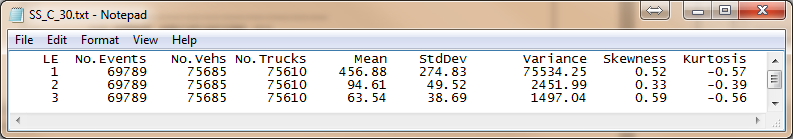
\includegraphics[width=6.5in,height=1.13958in]{media/image28.png}

\subsubsection*{Interval Statistics}\label{interval-statistics}
\addcontentsline{toc}{subsubsection}{Interval Statistics}

For intervals of specified duration (Line 51 of BTLSin.txt), the
statistics are recorded and written to disk when the buffer size is
exceeded (Line 41 of BTLSin.txt). This buffer size should be quite large
since not much memory is needed to store statistics. The files are
named:

SS\_S\_L\_Eff\_E.txt

Where \emph{L} is the bridge length and \emph{E} is the load effect
number. A sample output is shown below. The interval number and time are
also given.

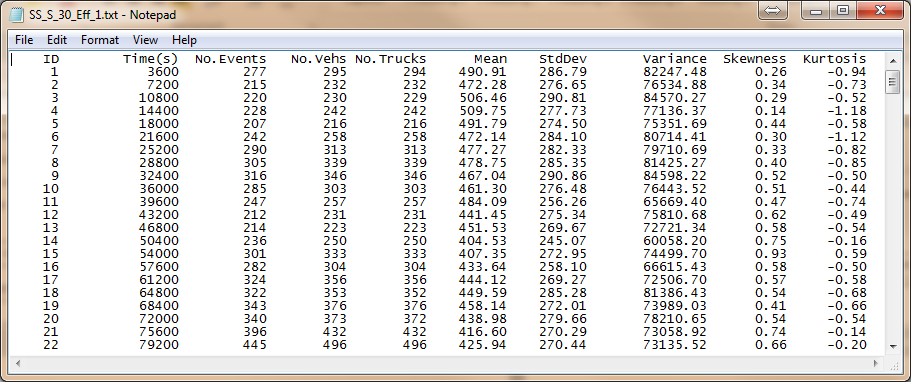
\includegraphics[width=6.5in,height=2.72083in]{media/image29.png}

\subsection{Loading Event File
Structure}\label{loading-event-file-structure}

This file structure contains all information relating to the event. An
example is shown below (from the Block Maximum Vehicle Files, Out by
Number of Trucks screenshot).

\begin{longtable}[]{@{}
  >{\raggedright\arraybackslash}p{(\linewidth - 2\tabcolsep) * \real{0.0899}}
  >{\raggedright\arraybackslash}p{(\linewidth - 2\tabcolsep) * \real{0.9101}}@{}}
\toprule\noalign{}
\endhead
\bottomrule\noalign{}
\endlastfoot
\textbf{Line} & \textbf{Data} \\
1 & 1 \\
2 & 1 1475.9 84395.5 17.58 2 \\
3 & 1001 1 1 023263466221 521119522 18 833315562 9413 9412 94 0 0 0 0 0
0 0 0 \\
4 & 1001 1 1 023263478251 593113511 18 8331167551151311513115 0 0 0 0 0
0 0 0 \\
5 & 2 409.0 84395.4 15.07 2 \\
6 & 1001 1 1 023263466221 521119522 18 833315562 9413 9412 94 0 0 0 0 0
0 0 0 \\
7 & 1001 1 1 023263478251 593113511 18 8331167551151311513115 0 0 0 0 0
0 0 0 \\
8 & 3 378.4 84395.3 12.56 2 \\
9 & 1001 1 1 023263466221 521119522 18 833315562 9413 9412 94 0 0 0 0 0
0 0 0 \\
10 & 1001 1 1 023263478251 593113511 18 8331167551151311513115 0 0 0 0 0
0 0 0 \\
11 & 2 \\
12 & 1 1198.8 100764.2 26.65 2 \\
13 & 1001 2 1 0 3592311240 449115511 18 683311857 8812 8813 88 0 0 0 0 0
0 0 0 \\
14 & 1001 2 1 0 3592372235 609108511 18 9429187561091010912109 0 0 0 0 0
0 0 0 \\
15 & 2 324.5 123199.1 -1.71 2 \\
16 & 1001 2 1 0101318 9222 219 61222 18 7461145 0 0 0 0 0 0 0 0 0 0 0 0
0 0 \\
17 & 1001 2 1 010131847242 600110511 1811030140581171211710117 0 0 0 0 0
0 0 0 \\
18 & 3 426.2 100764.2 26.65 2 \\
19 & 1001 2 1 0 3592311240 449115511 18 683311857 8812 8813 88 0 0 0 0 0
0 0 0 \\
20 & 1001 2 1 0 3592372235 609108511 18 9429187561091010912109 0 0 0 0 0
0 0 0 \\
\end{longtable}

Each line is explained as follows.

\paragraph*{Line 1:}\label{line-1-1}
\addcontentsline{toc}{paragraph}{Line 1:}

The index of the current block (if block maximum output), or the index
of the particular loading event in legacy files.

\paragraph*{Line 2:}\label{line-2-1}
\addcontentsline{toc}{paragraph}{Line 2:}

This is the load effect information line with 5 fields of data separated
by tabs:

\begin{itemize}
\item
  Field 1: The load effect number;
\item
  Field 2: The value of the load effect;
\item
  Field 3: The time at which this load effect was found in seconds;
\item
  Field 4: The distance of the first axle of the first truck on the
  bridge relative to the bridge datum, at the time of the crossing event
  maximum effect being reached. This allows one to sketch the positions
  of the trucks at the time of the load effect.
\item
  Field 5: The number of trucks comprising the event.
\end{itemize}

\paragraph*{Line 3-4:}\label{line-3-4}
\addcontentsline{toc}{paragraph}{Line 3-4:}

These lines provide the truck data string in CASTOR format for later
processing.

\paragraph*{Line 5+:}\label{line-5-1}
\addcontentsline{toc}{paragraph}{Line 5+:}

The format of lines 2-4 continues for each of the effects calculated.
Line 11 then provides the information for the start of the second block
or loading event, and the format repeats itself.

\section{Appendices}\label{appendices}

\subsection{Appendix 1 -- Traffic File
Formats}\label{appendix-1-traffic-file-formats}

\subsubsection*{\texorpdfstring{CASTOR File Format
}{CASTOR File Format }}\label{castor-file-format}
\addcontentsline{toc}{subsubsection}{CASTOR File Format }

In the table below, the Format column gives the storage type of the
data. IX refers to an integer of X number of digits, including leading
or trailing zeros.

\begin{longtable}[]{@{}
  >{\raggedright\arraybackslash}p{(\linewidth - 4\tabcolsep) * \real{0.6110}}
  >{\centering\arraybackslash}p{(\linewidth - 4\tabcolsep) * \real{0.1565}}
  >{\centering\arraybackslash}p{(\linewidth - 4\tabcolsep) * \real{0.2325}}@{}}
\toprule\noalign{}
\begin{minipage}[b]{\linewidth}\centering
\textbf{Record}
\end{minipage} & \begin{minipage}[b]{\linewidth}\centering
\textbf{Unit}
\end{minipage} & \begin{minipage}[b]{\linewidth}\centering
\textbf{Format}
\end{minipage} \\
\midrule\noalign{}
\endhead
\bottomrule\noalign{}
\endlastfoot
Head & & I4 \\
Day & & I2 \\
Month & & I2 \\
Year & & I2 \\
Hour & & I2 \\
Minute & & I2 \\
Second & & I2 \\
Second/100 & & I2 \\
Speed & dm/s & I3 \\
Gross Vehicle Weight - GVW & kg/100 & I4 \\
Length & dm & I3 \\
Number of Axles & & I1 \\
Direction (1 or 2) & & I1 \\
Lane & & I1 \\
Transverse Location In Lane & dm & I3 \\
Weight Axle 1 & kg/100 & I3 \\
Spacing Axle 1 - Axle 2 & dm & I2 \\
Weight Axle 2 & kg/100 & I3 \\
Spacing Axle 2 - Axle 3 & dm & I2 \\
$\vdots$
&
$\vdots$
&
$\vdots$ \\
Spacing Axle 8 - Axle 9 & dm & I2 \\
Weight Axle 9 & kg/100 & I3 \\
\end{longtable}

\subsubsection*{\texorpdfstring{\hfill\break
BeDIT File Format }{ BeDIT File Format }}\label{bedit-file-format}
\addcontentsline{toc}{subsubsection}{\hfill\break
BeDIT File Format }

This file format is similar to CASTOR except that the maximum number of
axles possible is 20, the axle spacings are given by a three digit
number, and the direction is zero-based.

\begin{longtable}[]{@{}
  >{\raggedright\arraybackslash}p{(\linewidth - 4\tabcolsep) * \real{0.6110}}
  >{\centering\arraybackslash}p{(\linewidth - 4\tabcolsep) * \real{0.1565}}
  >{\centering\arraybackslash}p{(\linewidth - 4\tabcolsep) * \real{0.2325}}@{}}
\toprule\noalign{}
\begin{minipage}[b]{\linewidth}\centering
\textbf{Record}
\end{minipage} & \begin{minipage}[b]{\linewidth}\centering
\textbf{Unit}
\end{minipage} & \begin{minipage}[b]{\linewidth}\centering
\textbf{Format}
\end{minipage} \\
\midrule\noalign{}
\endhead
\bottomrule\noalign{}
\endlastfoot
Head & & I4 \\
Day & & I2 \\
Month & & I2 \\
Year & & I2 \\
Hour & & I2 \\
Minute & & I2 \\
Second & & I2 \\
Second/100 & & I2 \\
Speed & dm/s & I3 \\
Gross Vehicle Weight - GVW & kg/100 & I4 \\
Length & dm & I3 \\
Number of Axles & & I2 \\
Direction (zero-based) & & I1 \\
Lane & & I1 \\
Transverse Location In Lane & dm & I3 \\
Weight Axle 1 & kg/100 & I3 \\
Spacing Axle 1 - Axle 2 & dm & I3 \\
Weight Axle 2 & kg/100 & I3 \\
Spacing Axle 2 - Axle 3 & dm & I3 \\
$\vdots$
&
$\vdots$
&
$\vdots$ \\
Spacing Axle 19 - Axle 20 & dm & I3 \\
Weight Axle 20 & kg/100 & I3 \\
\end{longtable}

\subsubsection*{\texorpdfstring{\hfill\break
DITIS File Format }{ DITIS File Format }}\label{ditis-file-format}
\addcontentsline{toc}{subsubsection}{\hfill\break
DITIS File Format }

This file format is similar to BeDIT except that the wheel track width
(i.e. transverse width of the vehicle, wheel-to-wheel) is included for
each axle; the transverse positon units are cm; and the direction is
one-based. This is for use with influence surfaces. Further, the year is
a four-digit number.

\begin{longtable}[]{@{}
  >{\centering\arraybackslash}p{(\linewidth - 8\tabcolsep) * \real{0.1272}}
  >{\raggedright\arraybackslash}p{(\linewidth - 8\tabcolsep) * \real{0.4457}}
  >{\centering\arraybackslash}p{(\linewidth - 8\tabcolsep) * \real{0.1208}}
  >{\centering\arraybackslash}p{(\linewidth - 8\tabcolsep) * \real{0.1532}}
  >{\centering\arraybackslash}p{(\linewidth - 8\tabcolsep) * \real{0.1532}}@{}}
\toprule\noalign{}
\begin{minipage}[b]{\linewidth}\centering
\textbf{Field}
\end{minipage} & \begin{minipage}[b]{\linewidth}\centering
\textbf{Record}
\end{minipage} & \begin{minipage}[b]{\linewidth}\centering
\textbf{Unit}
\end{minipage} & \begin{minipage}[b]{\linewidth}\centering
\textbf{Format}
\end{minipage} & \begin{minipage}[b]{\linewidth}\centering
\textbf{Start}
\end{minipage} \\
\midrule\noalign{}
\endhead
\bottomrule\noalign{}
\endlastfoot
1 & Head & & I4 & 1 \\
2 & Day & & I2 & 5 \\
3 & Month & & I2 & 7 \\
4 & Year & & I4 & 9 \\
5 & Hour & & I2 & 13 \\
6 & Minute & & I2 & 15 \\
7 & Second & & I2 & 17 \\
8 & Second/100 & & I2 & 19 \\
9 & Speed & dm/s & I3 & 21 \\
10 & Gross Vehicle Weight - GVW & kg/100 & I4 & 24 \\
11 & Length & dm & I3 & 28 \\
12 & Number of Axles & & I2 & 31 \\
13 & Direction (1 or 2) & & I1 & 33 \\
14 & Lane & & I1 & 34 \\
15 & Transverse Location In Lane & cm & I3 & 35 \\
16 & Weight Axle 1 & kg/100 & I3 & 38 \\
17 & Track Width Axle 1 & cm & I3 & 41 \\
18 & Spacing Axle 1 - Axle 2 & dm & I3 & 44 \\
19 & Weight Axle 2 & kg/100 & I3 & 47 \\
20 & Track Width Axle 2 & cm & I3 & 50 \\
21 & Spacing Axle 2 - Axle 3 & dm & I3 & 53 \\
$\vdots$
&
$\vdots$
&
$\vdots$
&
$\vdots$
&
$\vdots$ \\
72 & Spacing Axle 19 - Axle 20 & dm & I3 & 206 \\
73 & Weight Axle 20 & kg/100 & I3 & 209 \\
74 & Track Width Axle 20 & cm & I3 & 212 \\
\end{longtable}

\subsubsection*{\texorpdfstring{MON File Format
}{MON File Format }}\label{mon-file-format}
\addcontentsline{toc}{subsubsection}{MON File Format }

This file format is roughly similar to the BeDIT format but the units,
order, and number of digits in each field varies to match common
Australian WIM measurements. There is no defined maximum number of
axles, but the last axle spacing is defined, allowing calculation (from
the vehicle length) of the front and rear overhangs.

\begin{longtable}[]{@{}
  >{\raggedright\arraybackslash}p{(\linewidth - 4\tabcolsep) * \real{0.6110}}
  >{\centering\arraybackslash}p{(\linewidth - 4\tabcolsep) * \real{0.1565}}
  >{\centering\arraybackslash}p{(\linewidth - 4\tabcolsep) * \real{0.2325}}@{}}
\toprule\noalign{}
\begin{minipage}[b]{\linewidth}\centering
\textbf{Record}
\end{minipage} & \begin{minipage}[b]{\linewidth}\centering
\textbf{Unit}
\end{minipage} & \begin{minipage}[b]{\linewidth}\centering
\textbf{Format}
\end{minipage} \\
\midrule\noalign{}
\endhead
\bottomrule\noalign{}
\endlastfoot
Head & & I9 \\
Day & & I2 \\
Month & & I2 \\
Year & & I4 \\
Hour & & I2 \\
Minute & & I2 \\
Second & ms & I5 \\
Number of axles & & I2 \\
Number of axle groups & & I2 \\
Gross Vehicle Weight - GVW & kg & I6 \\
Speed & km/h & I3 \\
Length & mm & I5 \\
Lane (1-based local) & & I1 \\
Direction (0-based) & & I1 \\
Transverse Location In Lane & mm & I4 \\
Weight Axle 1 & kg & I5 \\
Spacing Axle 1 - Axle 2 & mm & I5 \\
Weight Axle 2 & kg & I5 \\
Spacing Axle 2 - Axle 3 & mm & I5 \\
$\vdots$
&
$\vdots$
&
$\vdots$ \\
Weight Axle -- Maximum defined & kg & I5 \\
Spacing Axle -- Maximum defined & mm & I5 \\
\end{longtable}

\subsubsection*{\texorpdfstring{SiWIM CSV File Format
}{SiWIM CSV File Format }}\label{siwim-csv-file-format}
\addcontentsline{toc}{subsubsection}{SiWIM CSV File Format }

Introduced in v1.3.7, this format (format code 5) reads the CSV export
of the SiWIM\textsuperscript{®} bridge weigh-in-motion system. Unlike
the fixed-width formats above, it is a comma-separated file whose
first line is a header row; columns are located by header name, so the
column order is not fixed and unrecognised columns are ignored. This
format is \textbf{read-only}: it cannot be selected as the vehicle
output file format.

The columns used by BTLS are:

\begin{longtable}[]{@{}
  >{\raggedright\arraybackslash}p{(\linewidth - 4\tabcolsep) * \real{0.28}}
  >{\raggedright\arraybackslash}p{(\linewidth - 4\tabcolsep) * \real{0.12}}
  >{\raggedright\arraybackslash}p{(\linewidth - 4\tabcolsep) * \real{0.60}}@{}}
\toprule\noalign{}
\begin{minipage}[b]{\linewidth}\raggedright
\textbf{Header name}
\end{minipage} & \begin{minipage}[b]{\linewidth}\raggedright
\textbf{Unit}
\end{minipage} & \begin{minipage}[b]{\linewidth}\raggedright
\textbf{Description}
\end{minipage} \\
\midrule\noalign{}
\endhead
\bottomrule\noalign{}
\endlastfoot
\texttt{wim.ts} & & Timestamp, \texttt{YYYY-MM-DD-HH-MM-SS-mmm}
(millisecond resolution) \\
\texttt{wim.lane} & & Lane number, 1-based local (defaults to 1 if
absent); all vehicles are assigned direction 1 \\
\texttt{wim.v} & m/s & Vehicle velocity \\
\texttt{wim.naxles} & & Number of axles (must be at least 1) \\
\texttt{wim.axgrps} & & Axle group pattern, e.g.\ \texttt{1233} for a
9-axle vehicle in 4 groups; the number of groups is taken as the
number of digits. If absent or invalid, groups are inferred from the
axle spacings (a spacing greater than 2.0~m starts a new group) \\
\texttt{wim.gvw} & kN & Gross vehicle weight \\
\texttt{wim.whlbse} & m & Wheelbase; used as the vehicle length \\
\texttt{wim.acws.w.\emph{i}} & kN & Weight of axle \emph{i}
(0-based), for $i = 0 \ldots \texttt{naxles}-1$ \\
\texttt{wim.ads.d.\emph{i}} & m & Spacing between axle \emph{i} and
axle $i+1$ (0-based) \\
\end{longtable}

The transverse position in lane is not present in the SiWIM export and
is set to zero. The first line of the file must be the header row; a
file without a header, a bad timestamp, or a row with an invalid axle
count is reported as an input error.

\subsection{Appendix 2 -- References}\label{appendix-2-references}

\begin{itemize}
\item
  Caprani, C.C. (2005), \emph{Probabilistic Analysis of Highway Bridge
  Traffic Loading}, PhD Thesis, School of Architecture, Landscape and
  Civil Engineering, University College Dublin, Ireland.
  \url{http://www.colincaprani.com/research/phd-dissertation/}
\item
  Caprani, C.C. (2012), `Calibration of a congestion load model for
  highway bridges using traffic microsimulation', \emph{Structural
  Engineering International}, 22(3), August, in print.
\item
  Caprani, C.C., OBrien, E.J. and McLachlan, G.J. (2008),
  `Characteristic traffic load effects from a mixture of loading events
  on short to medium span bridges', \emph{Structural Safety}, Vol.
  30(5), September, pp. 394-404.
\end{itemize}

\begin{quote}
\href{http://www.colincaprani.com/wordpress/go.php?http://dx.doi.org/10.1016/j.strusafe.2006.11.006}{10.1016/j.strusafe.2006.11.006}
\end{quote}

\begin{itemize}
\item
  Grave, S.A.J. (2001), \emph{Modelling of Site-Specific Traffic Loading
  on Short to Medium Span Bridges}, Ph.D. Thesis, Department of Civil
  Engineering, Trinity College Dublin.
\item
  OBrien, E.J. and Caprani, C.C. (2005), `Headway modelling for traffic
  load assessment of short- to medium-span bridges', \emph{The
  Structural Engineer}, Vol 83, No. 16, August, pp. 33-36.
\end{itemize}

\begin{quote}
\href{http://www.colincaprani.com/wordpress/go.php?http://www.istructe.org/thestructuralengineer/HC/Abstract.asp?PID=5494}{http://www.istructe.org/thestructuralengineer/HC/Abstract.asp?PID=5494}
\end{quote}

\end{document}
